\section{RNA-Seq}
\subsection{概述}
\begin{frame}
  \frametitle{转录组学 | RNA-Seq | 简介}
  \begin{figure}
    \centering
    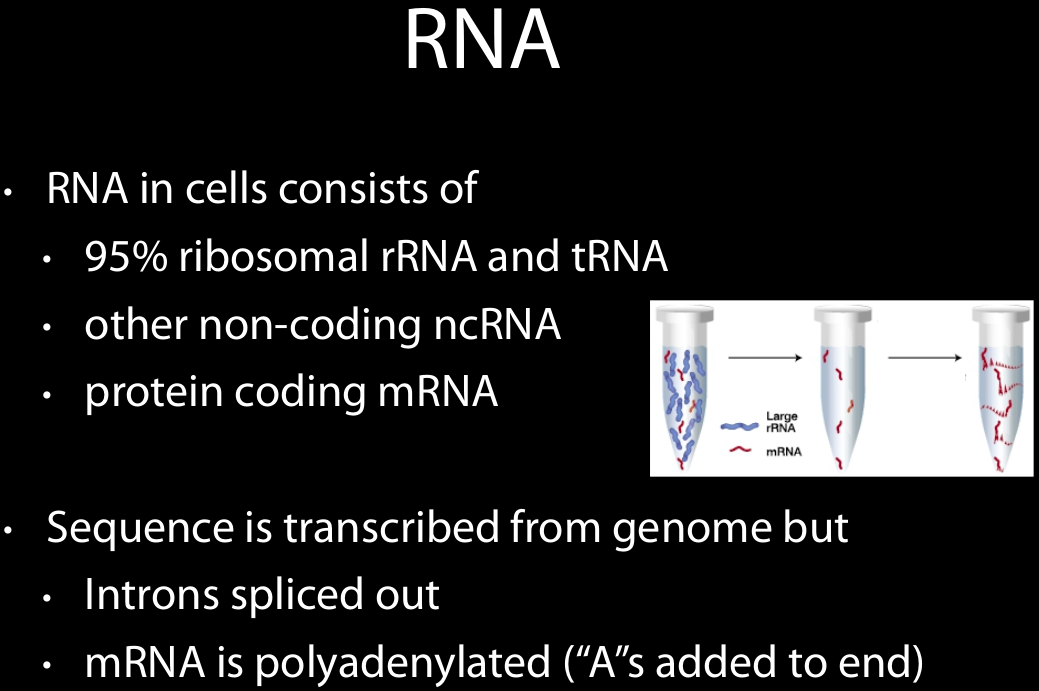
\includegraphics[width=0.9\textwidth]{c3_transcriptome/rna_01.png}
  \end{figure}
\end{frame}

\begin{frame}
  \frametitle{转录组学 | RNA-Seq | 简介}
  \begin{block}{\textcolor{red}{RNA-Seq}}
 RNA测序(RNA sequencing,简称RNA-Seq,也被称为全转录物组鸟枪法测序,Whole Transcriptome Shotgun Sequencing,简称WTSS)是基于第二代测序技术的转录组学研究方法。RNA测序是使用第二代测序的能力,在给定时刻从一个基因组中,揭示RNA的存在和数量的一个快照的技术。\\
 \vspace{1em}
RNA-seq (RNA sequencing), also called whole transcriptome shotgun sequencing (WTSS), uses next-generation sequencing (NGS) to reveal the presence and quantity of RNA in a biological sample at a given moment in time.
  \end{block}
\end{frame}

\begin{frame}
  \frametitle{转录组学 | RNA-Seq | Method | RNA Poly(A) library}
  \begin{block}{poly(A)-poly(T)}
    Frequently, in mRNA analysis the 3' polyadenylated (poly(A)) tail is targeted in order to ensure that coding RNA is separated from noncoding RNA. This can be accomplished simply with poly (T) oligos covalently attached to a given substrate. Presently many studies utilize magnetic beads for this step.
  \end{block}
  \pause
  \begin{block}{poly(T) \& rRNA}
    Studies including portions of the transcriptome outside poly(A) RNAs have shown that when using poly(T) magnetic beads, the flow-through RNA (non-poly(A) RNA) can yield important noncoding RNA gene discovery which would have otherwise gone unnoticed.\\
    \vspace{0.2em}
    Also, since ribosomal RNA represents over 90\% of the RNA within a given cell, studies have shown that its removal via probe hybridization increases the capacity to retrieve data from the remaining portion of the transcriptome.
  \end{block}
\end{frame}

\begin{frame}
  \frametitle{转录组学 | RNA-Seq | Method | Transcriptome assembly}
  \begin{block}{\textcolor{red}{Two methods}}
    Two different assembly methods are used for producing a transcriptome from raw sequence reads: genome-guided and \textit{de-novo}. 
  \end{block}
  \begin{figure}
    \centering
    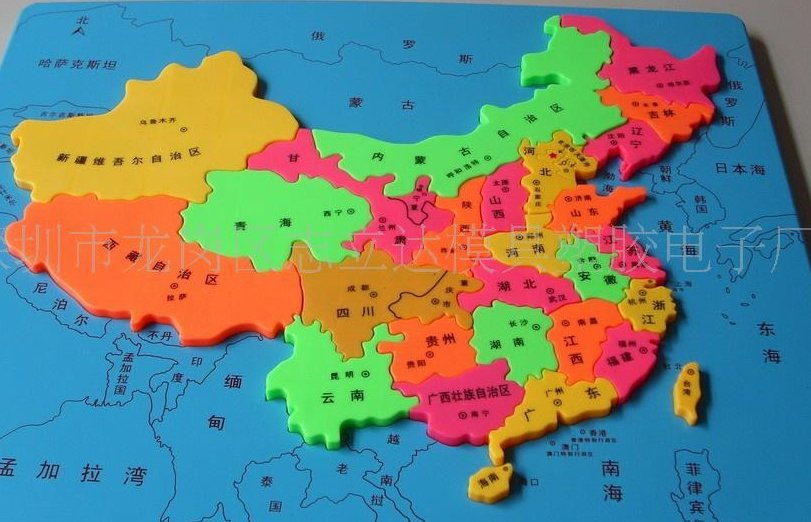
\includegraphics[width=0.42\textwidth]{c3_transcriptome/rs_method_denovo_01.jpg} \quad
    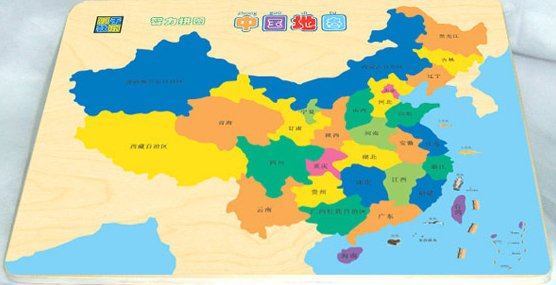
\includegraphics[width=0.53\textwidth]{c3_transcriptome/rs_method_guide_01.jpg}
  \end{figure}
\end{frame}

\begin{frame}
  \frametitle{转录组学 | RNA-Seq | Method | Transcriptome assembly}
  \begin{figure}
    \centering
    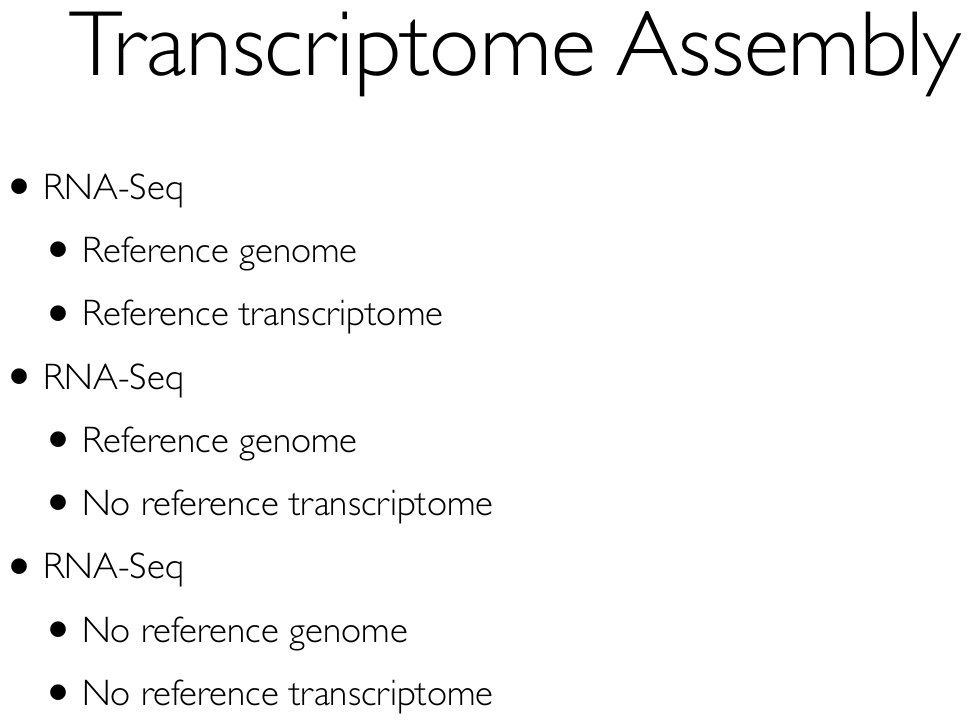
\includegraphics[width=0.8\textwidth]{c3_transcriptome/rs_method_00.png}
  \end{figure}
\end{frame}

\begin{frame}
  \frametitle{转录组学 | RNA-Seq | Method | Transcriptome assembly}
  \begin{figure}
    \centering
    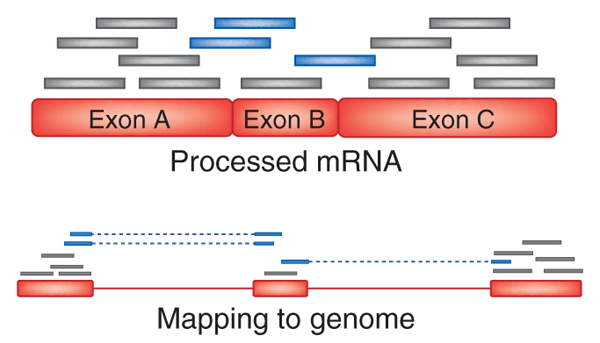
\includegraphics[width=0.9\textwidth]{c3_transcriptome/rs_method_guide_intron_02.png}
  \end{figure}
\end{frame}

\begin{frame}
  \frametitle{转录组学 | RNA-Seq | Method | Experimental considerations}
  {\footnotesize
  \begin{block}{pros \& cons}
    \begin{itemize}
      \item Tissue specificity: Gene expression is not uniform throughout an organism's cells, it is strongly dependent on the tissue type being measured. RNA-Seq can provide a complete snapshot of all the transcripts being available at that precise moment in the cell.
      \item Time dependent: During a cell's lifetime and context, its gene expression levels change. Any single sequencing experiment will offer information regarding one point in time.
      \item Coverage: coverage/depth can affect the mutations seen.
      \item Subjectivity of the analysis: Numerous attempts have been taken to uniformly analyze the data. However, the results can vary due to the multitude of algorithms and pipelines available.
      \item Data management: The main issue with NGS data is the volume of data produced.
      \item Downstream interpretation of the data: Different layers of interpretations have to be considered when analyzing RNA-Seq data.
    \end{itemize}
  \end{block}
  }
\end{frame}

\begin{frame}
  \frametitle{转录组学 | RNA-Seq | \textcolor{red}{Application}}
  \begin{figure}
    \centering
    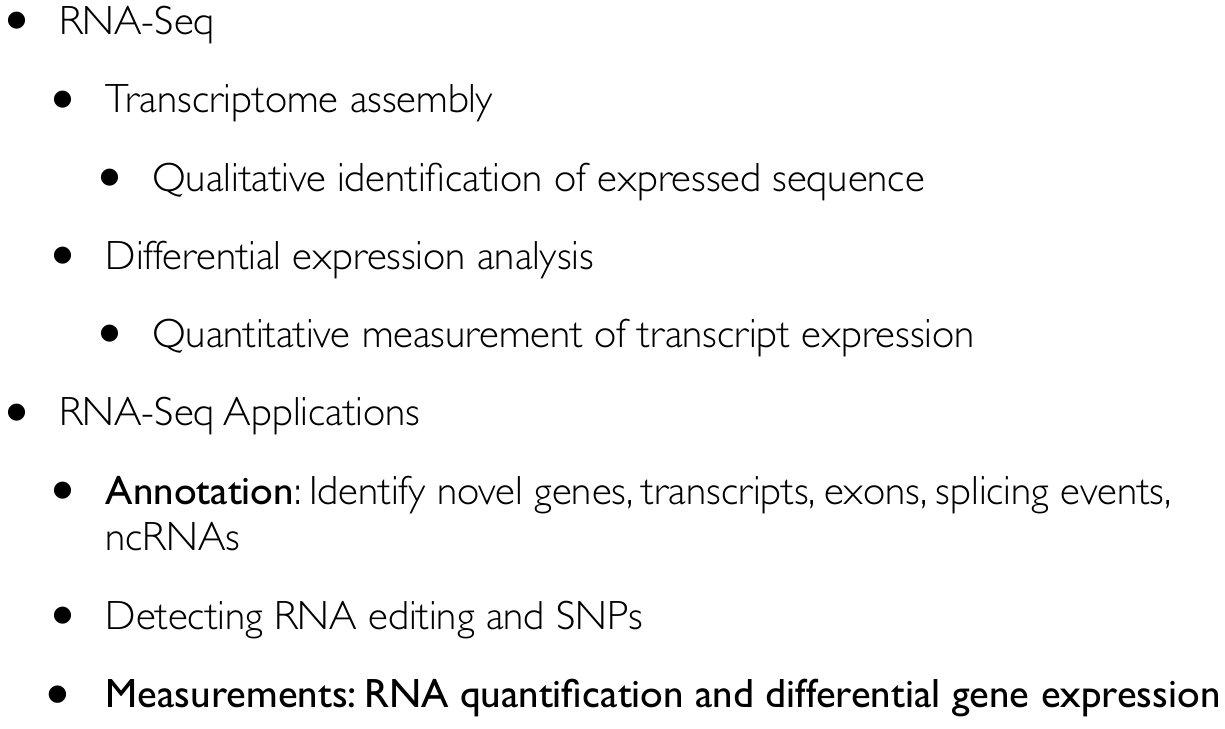
\includegraphics[width=0.9\textwidth]{c3_transcriptome/rs_application_00.png}
  \end{figure}
\end{frame}

\begin{frame}
  \frametitle{转录组学 | RNA-Seq | Application}
  \begin{figure}
    \centering
    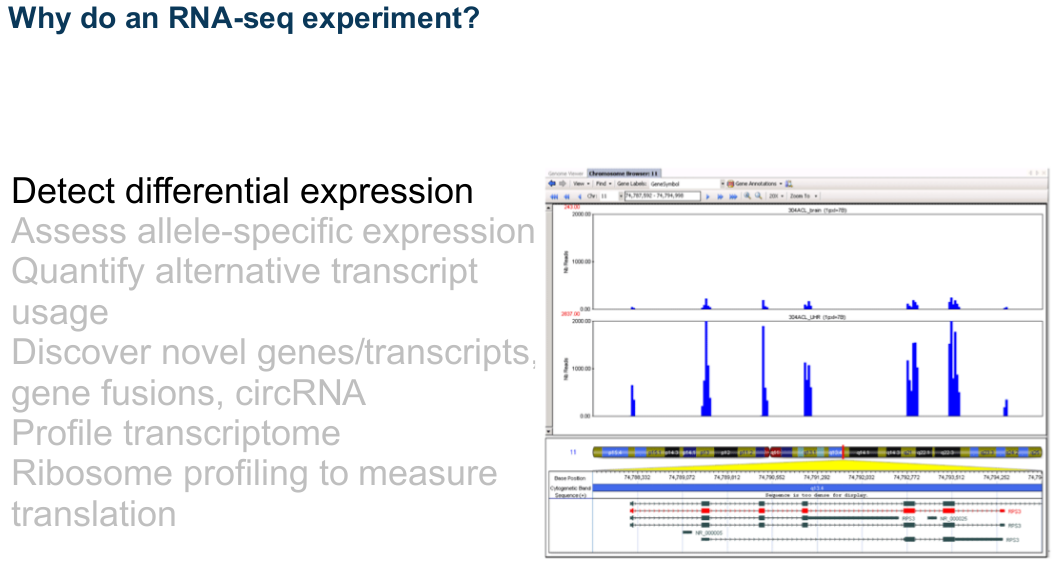
\includegraphics[width=0.9\textwidth]{c3_transcriptome/rs_application_10.png}
  \end{figure}
\end{frame}

\begin{frame}
  \frametitle{转录组学 | RNA-Seq | Application}
  \begin{figure}
    \centering
    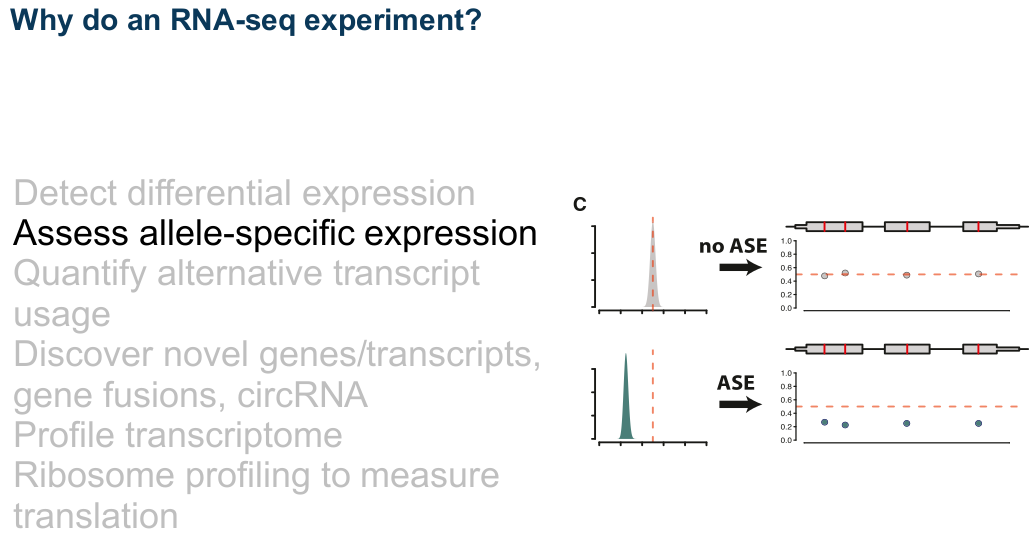
\includegraphics[width=0.9\textwidth]{c3_transcriptome/rs_application_11.png}
  \end{figure}
\end{frame}

\begin{frame}
  \frametitle{转录组学 | RNA-Seq | Application}
  \begin{figure}
    \centering
    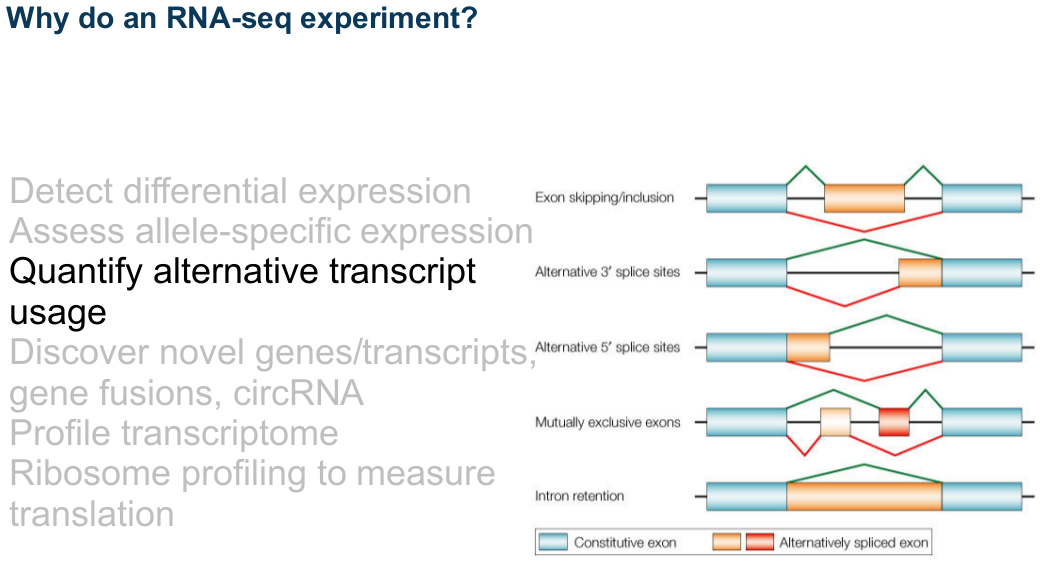
\includegraphics[width=0.9\textwidth]{c3_transcriptome/rs_application_12.png}
  \end{figure}
\end{frame}

\begin{frame}
  \frametitle{转录组学 | RNA-Seq | Application}
  \begin{figure}
    \centering
    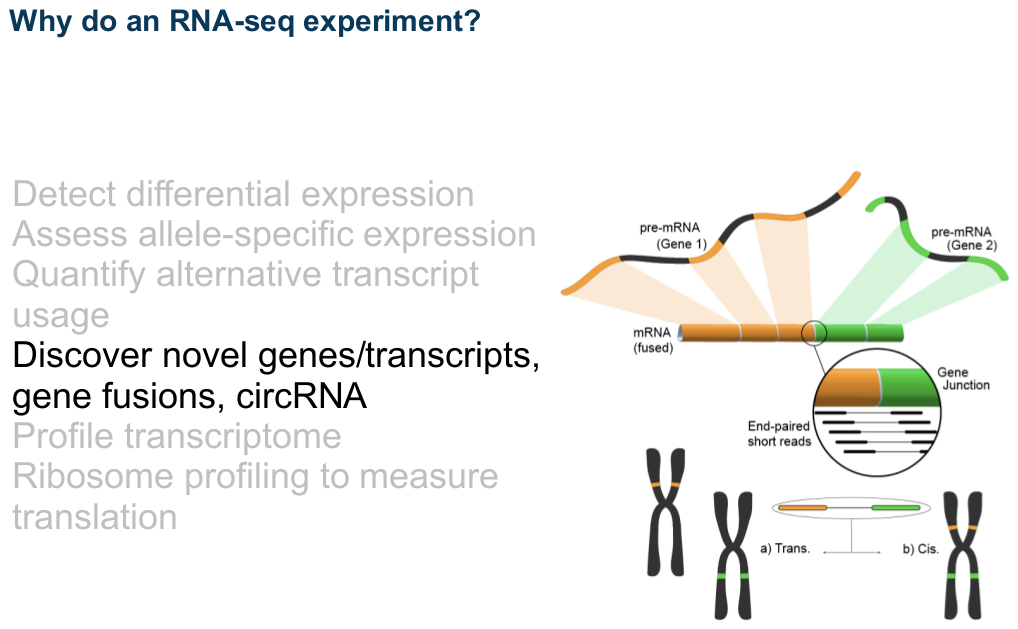
\includegraphics[width=0.9\textwidth]{c3_transcriptome/rs_application_13.png}
  \end{figure}
\end{frame}

\begin{frame}
  \frametitle{转录组学 | RNA-Seq | Application}
  \begin{figure}
    \centering
    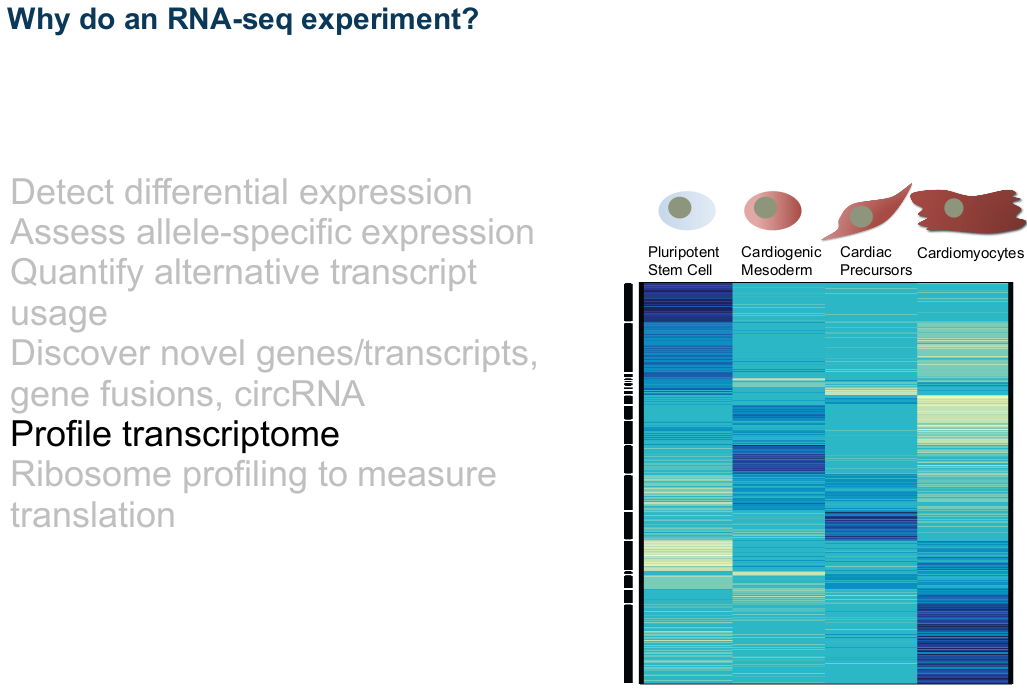
\includegraphics[width=0.9\textwidth]{c3_transcriptome/rs_application_14.png}
  \end{figure}
\end{frame}

\begin{frame}
  \frametitle{转录组学 | RNA-Seq | Application}
  \begin{figure}
    \centering
    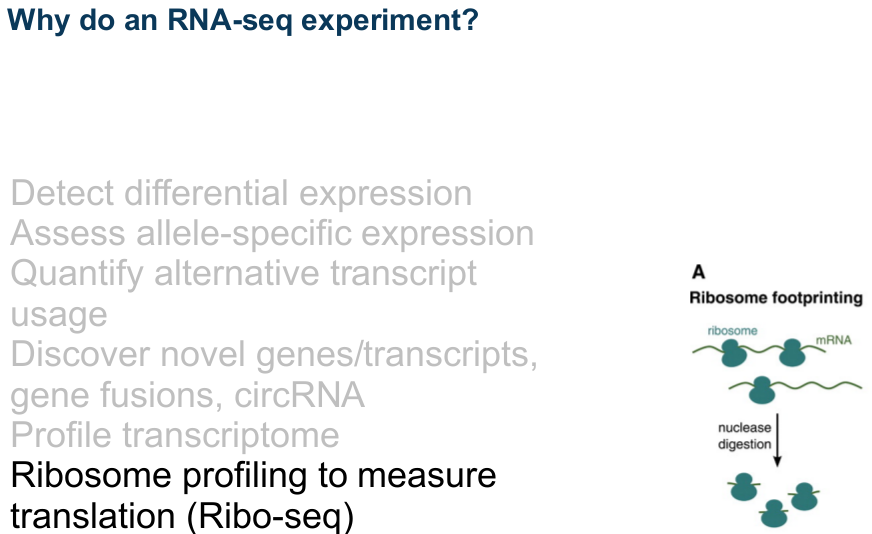
\includegraphics[width=0.9\textwidth]{c3_transcriptome/rs_application_15.png}
  \end{figure}
\end{frame}

\begin{frame}
  \frametitle{转录组学 | RNA-Seq | Experiment}
  \begin{figure}
    \centering
    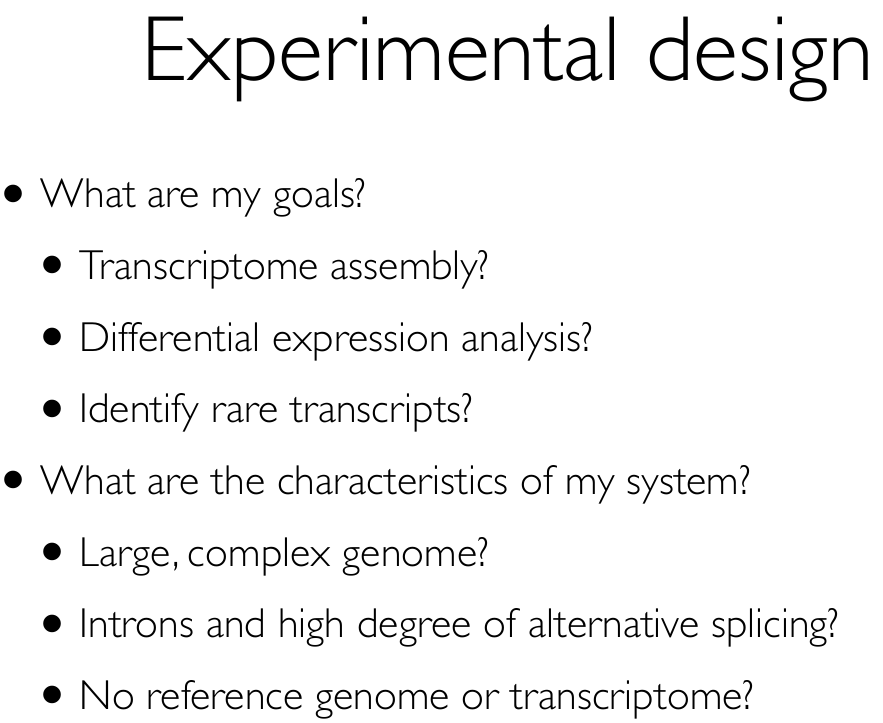
\includegraphics[width=0.8\textwidth]{c3_transcriptome/rs_experiment_01.png}
  \end{figure}
\end{frame}

\begin{frame}
  \frametitle{转录组学 | RNA-Seq | Analysis | \textcolor{red}{Workflow}}
  \begin{figure}
    \centering
    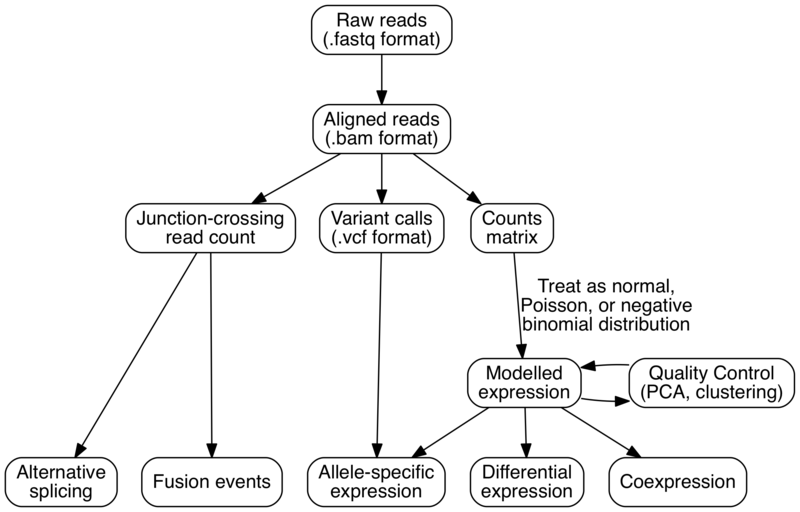
\includegraphics[width=0.9\textwidth]{c3_transcriptome/rs_analysis_workflow_01.png}
  \end{figure}
\end{frame}

\begin{frame}
  \frametitle{转录组学 | RNA-Seq | Analysis | Gene expression}
  \begin{figure}
    \centering
    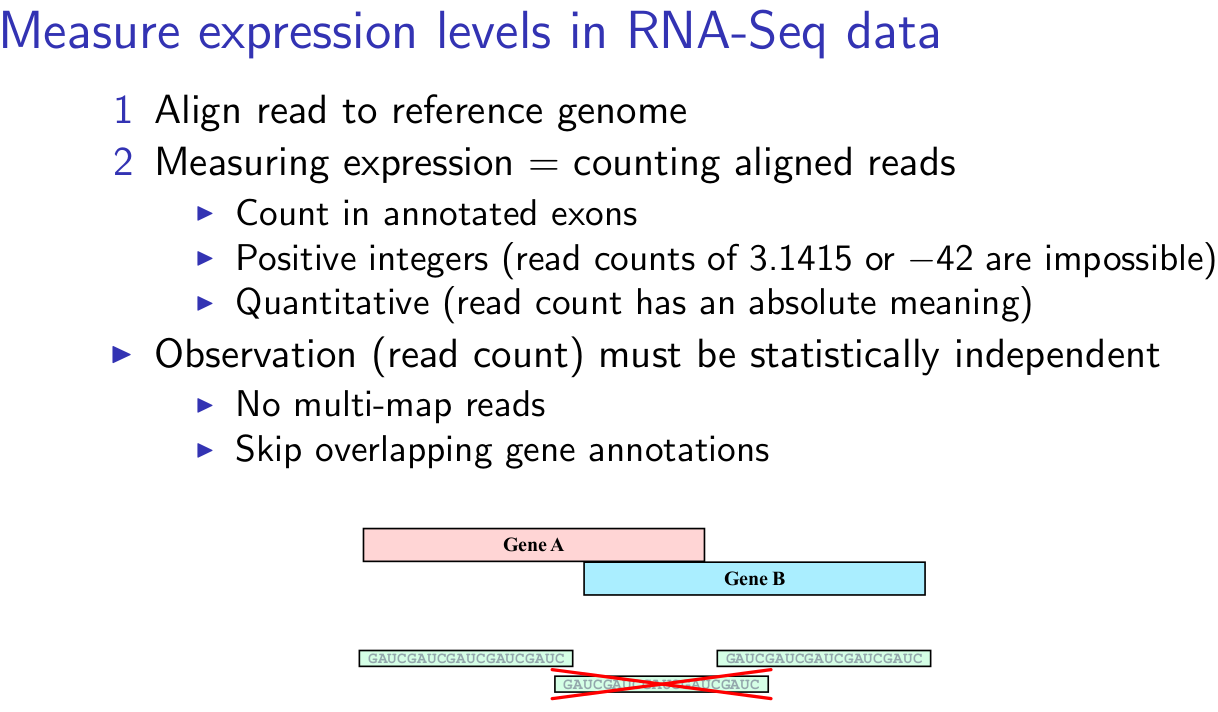
\includegraphics[width=\textwidth]{c3_transcriptome/rs_exp_01.png}
  \end{figure}
\end{frame}

\begin{frame}
  \frametitle{转录组学 | RNA-Seq | Analysis | Differential expression}
  \begin{figure}
    \centering
    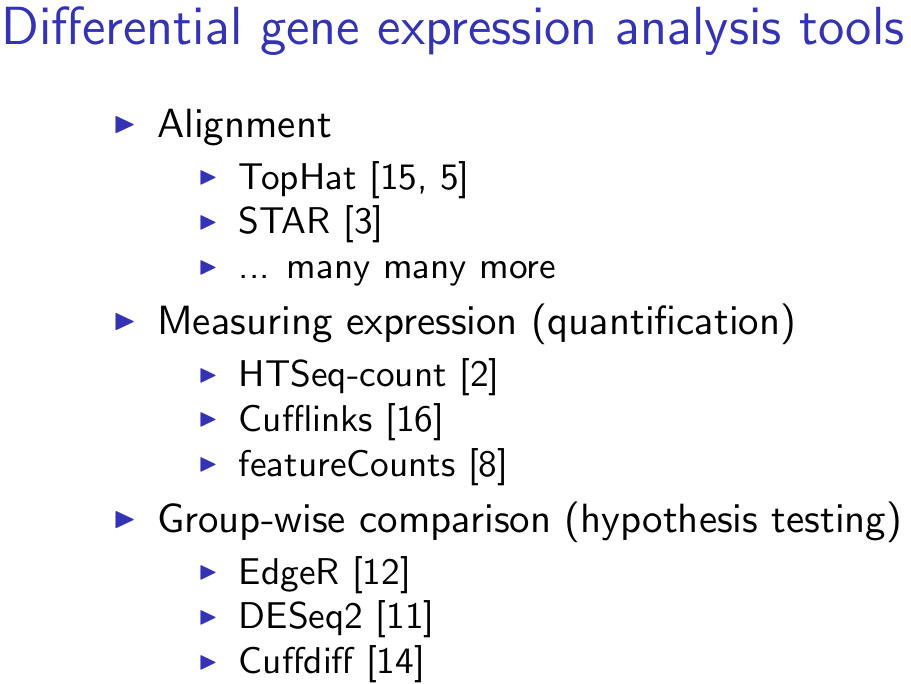
\includegraphics[width=0.85\textwidth]{c3_transcriptome/rs_deg_01.png}
  \end{figure}
\end{frame}

\begin{frame}
  \frametitle{转录组学 | RNA-Seq | Analysis | SNV discovery}
  \begin{figure}
    \centering
    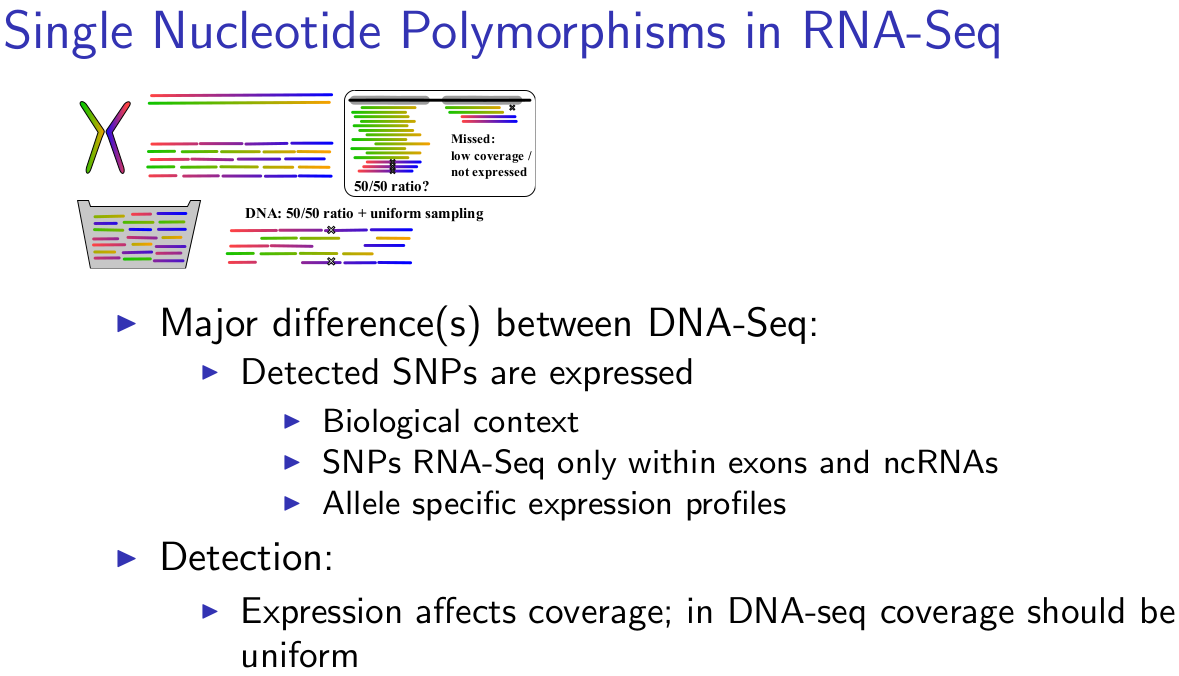
\includegraphics[width=0.9\textwidth]{c3_transcriptome/rs_snv_01.png}
  \end{figure}
\end{frame}

\begin{frame}
  \frametitle{转录组学 | RNA-Seq | Analysis | SNV discovery}
  \begin{figure}
    \centering
    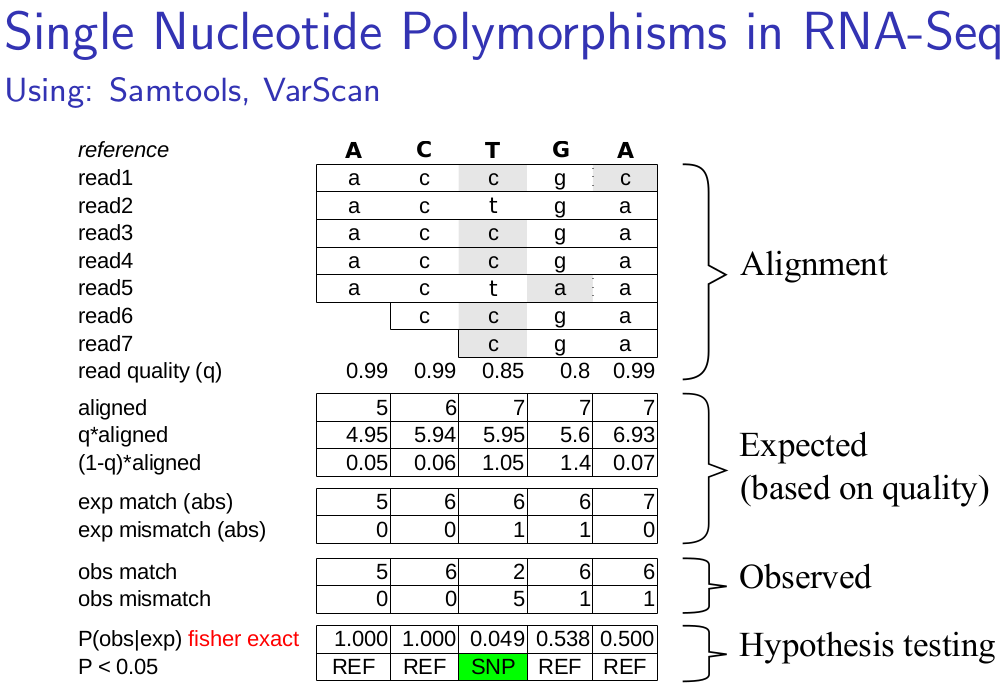
\includegraphics[width=0.9\textwidth]{c3_transcriptome/rs_snv_02.png}
  \end{figure}
\end{frame}

\begin{frame}
  \frametitle{转录组学 | RNA-Seq | Analysis | SNV discovery}
  \begin{figure}
    \centering
    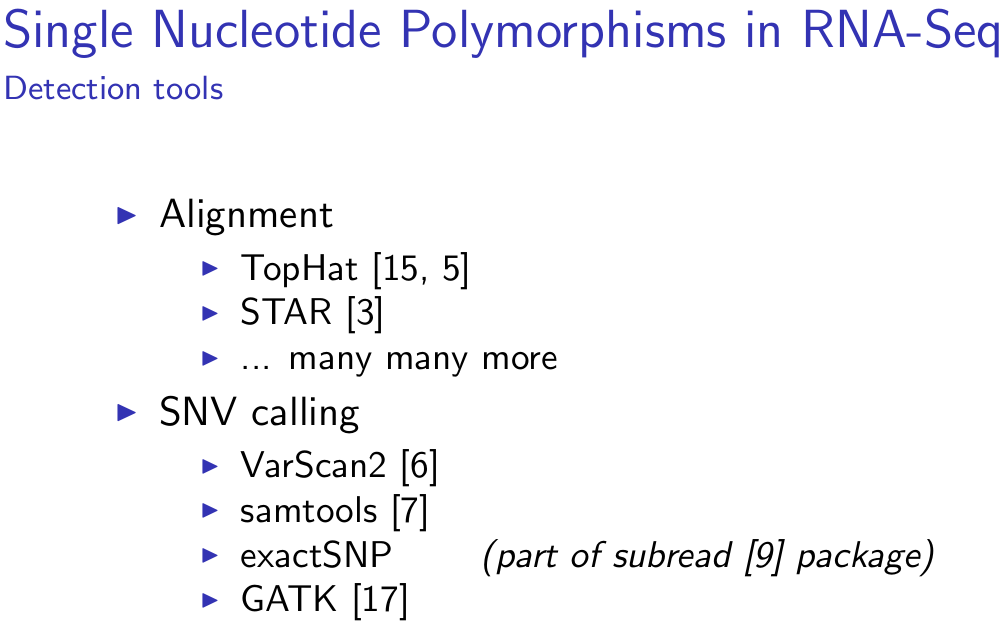
\includegraphics[width=0.9\textwidth]{c3_transcriptome/rs_snv_03.png}
  \end{figure}
\end{frame}

\begin{frame}
  \frametitle{转录组学 | RNA-Seq | Analysis | Fusion gene detection}
  \begin{figure}
    \centering
    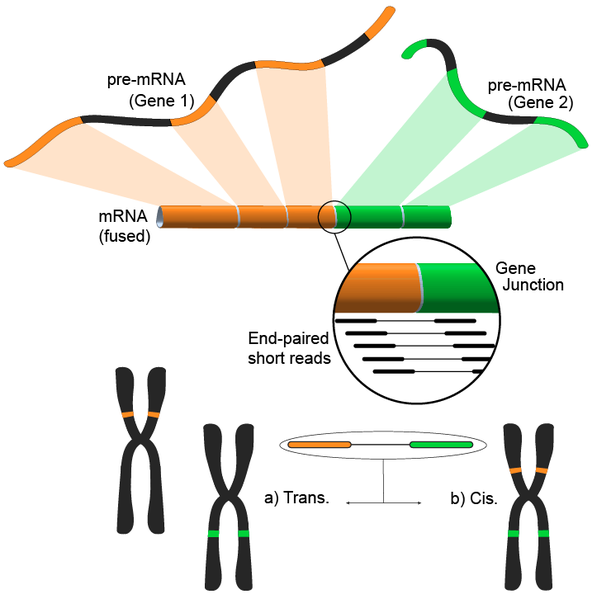
\includegraphics[width=0.6\textwidth]{c3_transcriptome/rs_analysis_fusion_01.png}
  \end{figure}
\end{frame}

\begin{frame}
  \frametitle{转录组学 | RNA-Seq | Databases}
  {\footnotesize
  \begin{block}{ENCODE}
    ENCODE aimed to identify genome-wide regulatory regions in different cohort of cell lines and transcriptomic data are paramount in order to understand the downstream effect of those epigenetic and genetic regulatory layers.
  \end{block}
  \pause
  \begin{block}{RNA Seq Atlas}
    RNA-Seq Atlas is a web-based repository of RNA-Seq gene expression profiles and query tools. The website offers free and easy access to RNA-Seq gene expression profiles and tools to both compare tissues and find genes with specific expression patterns.
  \end{block}
  \pause
  \begin{block}{TCGA}
    TCGA aimed to collect and analyze thousands of patient's samples from 30 different tumor types in order to understand the underlying mechanisms of malignant transformation and progression.
  \end{block}
}
\end{frame}

\begin{frame}
  \frametitle{转录组学 | RNA-Seq | Databases | ENCODE}
  \begin{block}{ENCODE}
 DNA元件百科全书(Encyclopedia of DNA Elements,简称为ENCODE项目)是一个由美国国家人类基因组研究所(NHGRI)在2003年9月发起的一项公共联合研究项目,旨在找出人类基因组中所有功能组件。这是继完成人类基因组计划后国家人类基因组研究所开始的最重要的项目之一。
  \end{block}
  \pause
  \begin{block}{三个阶段}
    \begin{itemize}
      \item 试验阶段:测试和比较现有方法以便严格分析一个所定义的人类基因组序列的一部分
      \item 技术发展阶段:分析整个基因组,并进行“额外中试规模研究”
      \item 生产阶段:2012年9月5日,该项目的初步结果被整理为30篇论文并同时发表于多个刊物,包括6篇论文在《自然》、6篇论文在《基因组生物学》及18篇论文在《基因组研究》上
    \end{itemize}
  \end{block}
\end{frame}

\subsection{数据分析}
\begin{frame}
  \frametitle{转录组学 | RNA-Seq | 分析 | \textcolor{red}{概览}}
  \begin{figure}
    \centering
    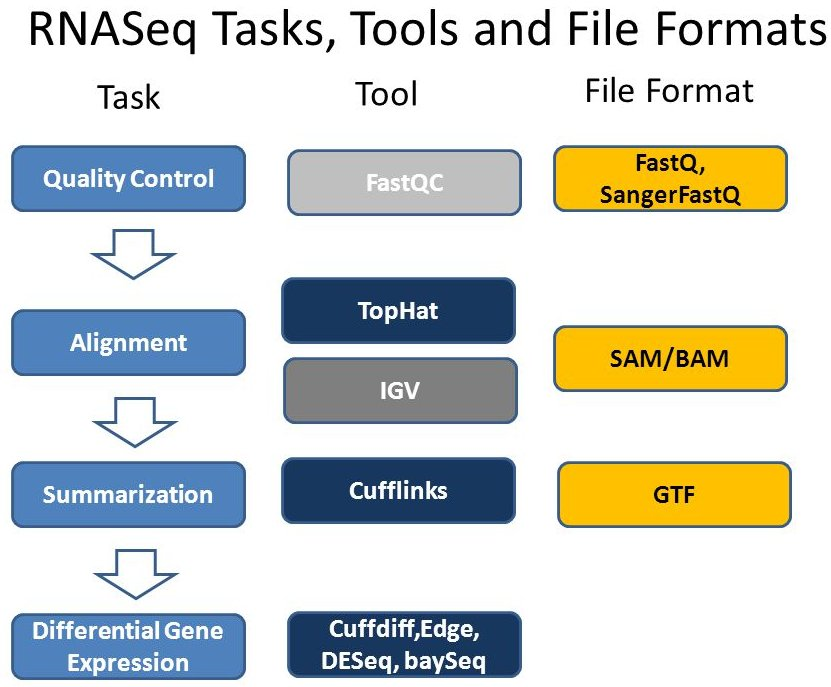
\includegraphics[width=0.8\textwidth]{c3_transcriptome/workflow_tool_format_01.jpg}
  \end{figure}
\end{frame}

\begin{frame}
  \frametitle{转录组学 | RNA-Seq | 分析 | \textcolor{red}{概览}}
  \begin{figure}
    \centering
    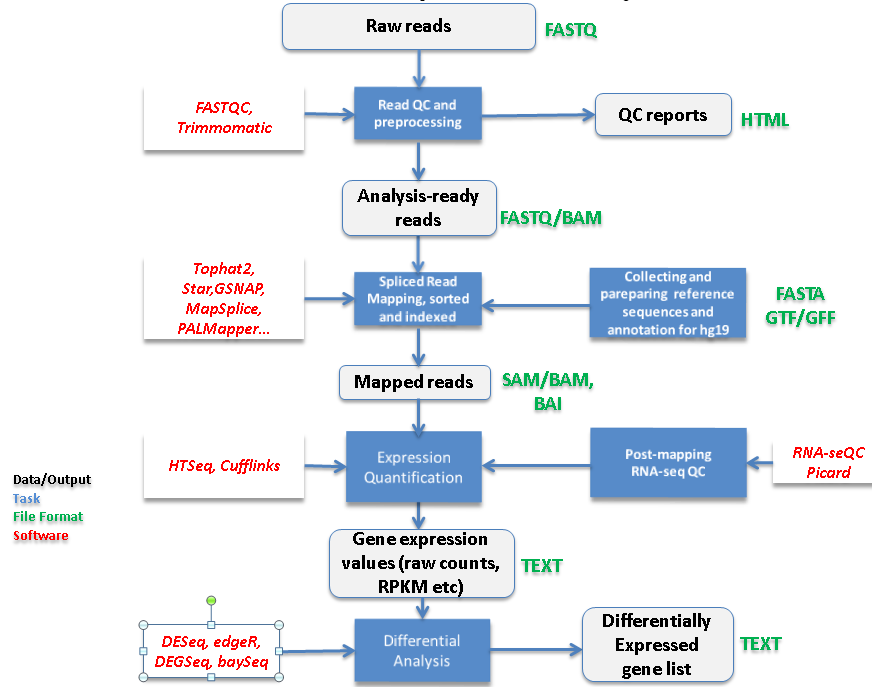
\includegraphics[width=0.8\textwidth]{c3_transcriptome/workflow_tool_format_02.png}
  \end{figure}
\end{frame}

\subsubsection{流程}
\begin{frame}
  \frametitle{转录组学 | RNA-Seq | 分析 | 流程}
  \begin{figure}
    \centering
    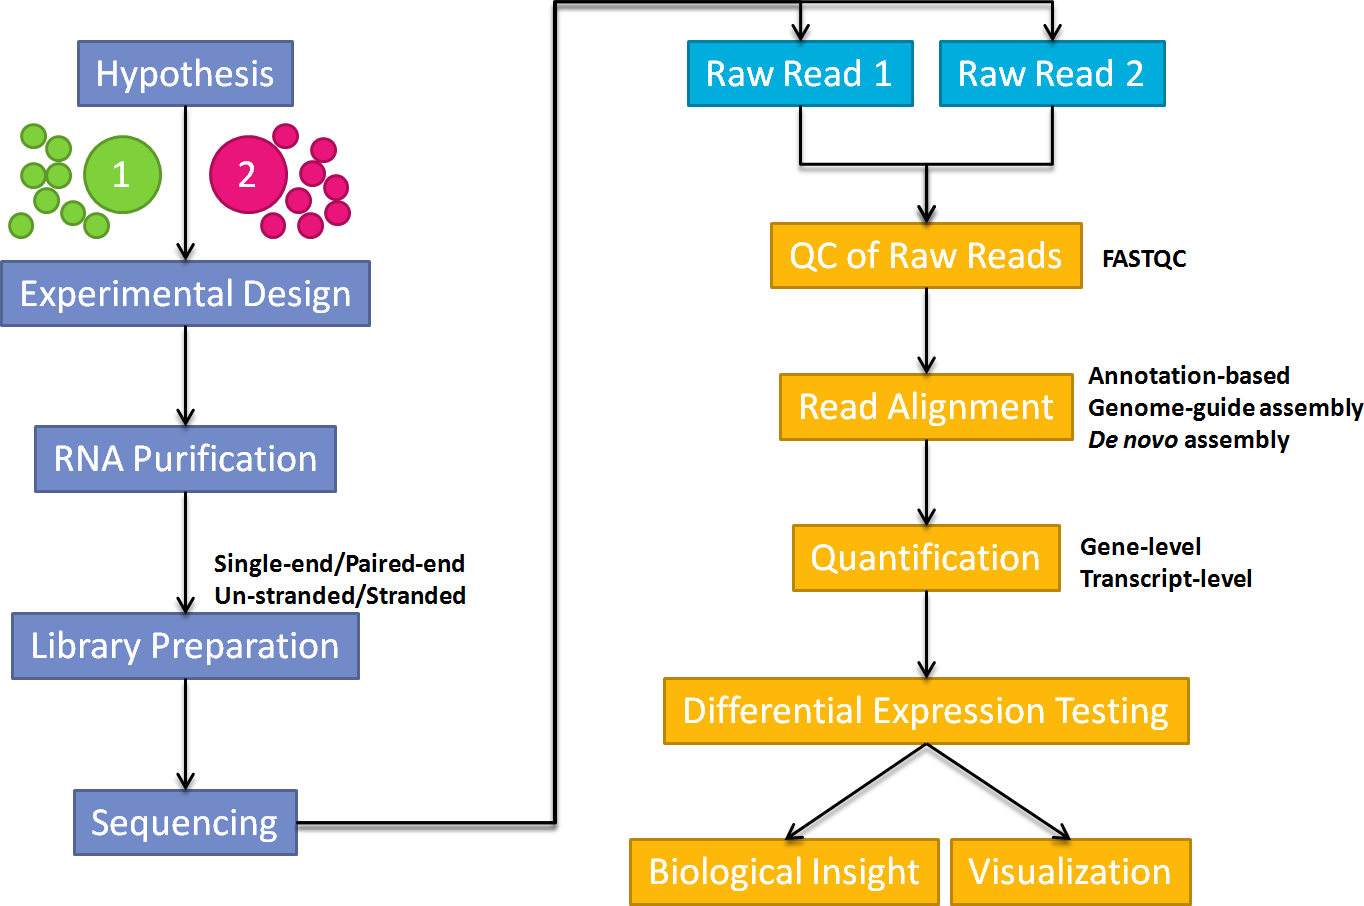
\includegraphics[width=0.9\textwidth]{c3_transcriptome/workflow_all_04.png}
  \end{figure}
\end{frame}

\begin{frame}
  \frametitle{转录组学 | RNA-Seq | 分析 | 流程}
  \begin{figure}
    \centering
    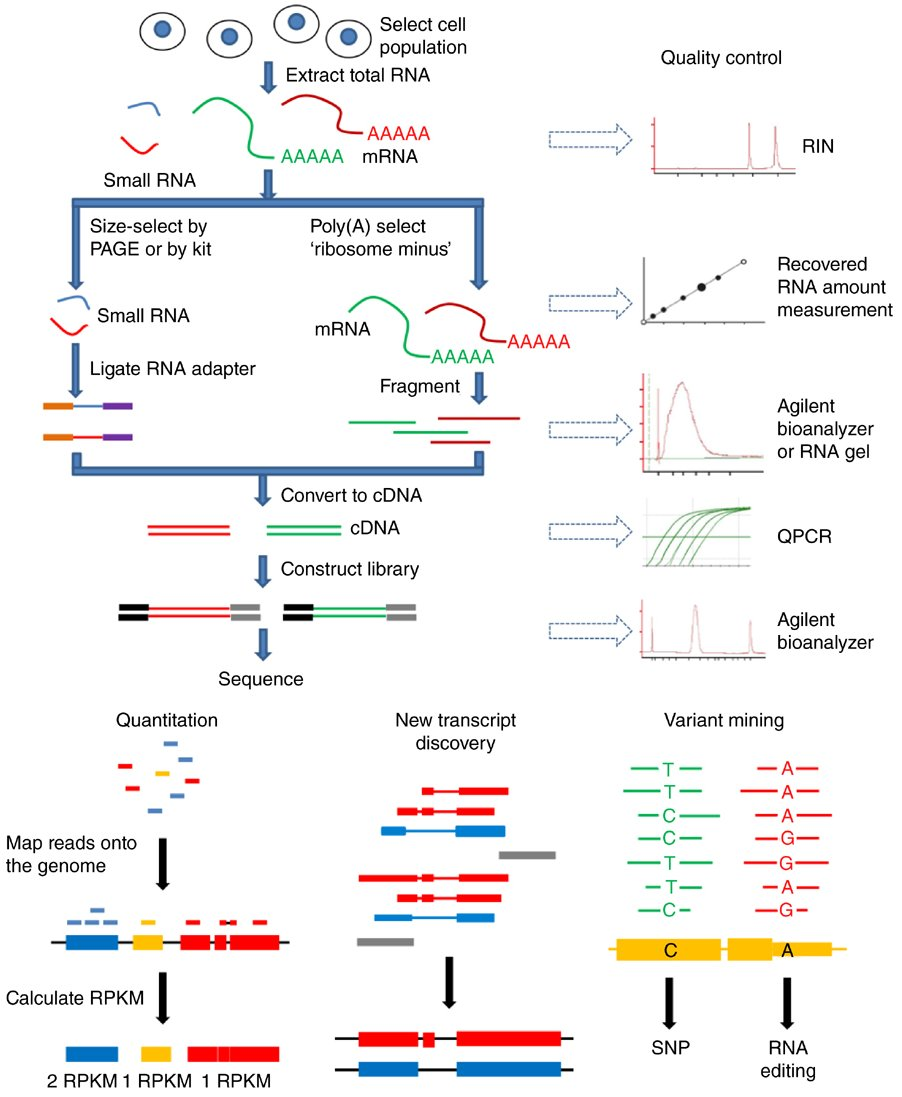
\includegraphics[width=0.53\textwidth]{c3_transcriptome/workflow_all_03.jpg}
  \end{figure}
\end{frame}

\begin{frame}
  \frametitle{转录组学 | RNA-Seq | 分析 | 流程 | 实验}
  \begin{figure}
    \centering
    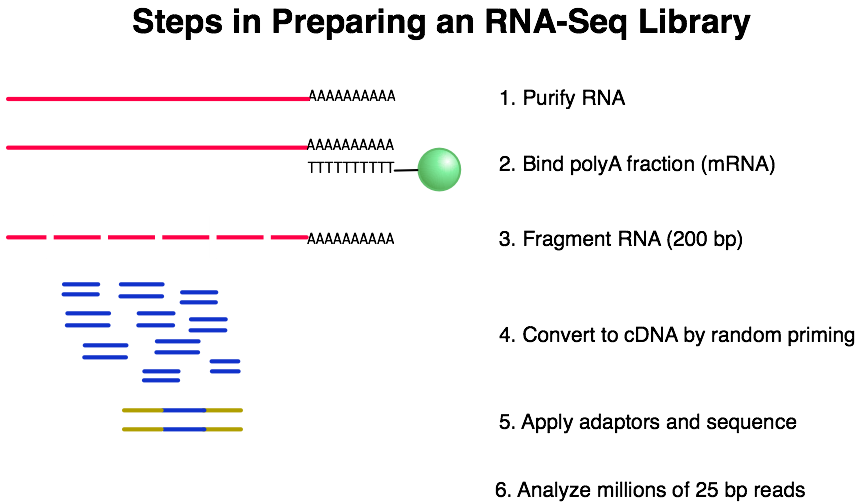
\includegraphics[width=0.9\textwidth]{c3_transcriptome/workflow_exp_01.png}
  \end{figure}
\end{frame}

\begin{frame}
  \frametitle{转录组学 | RNA-Seq | 分析 | 流程 | 实验}
  \begin{figure}
    \centering
    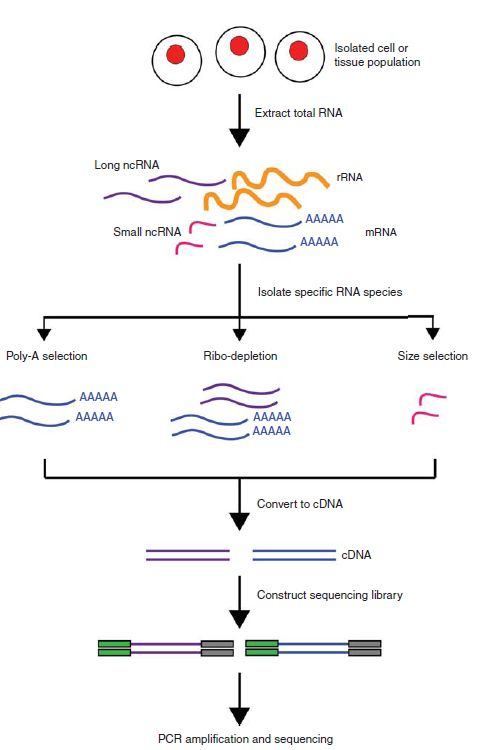
\includegraphics[width=0.4\textwidth]{c3_transcriptome/workflow_exp_02.jpg}
  \end{figure}
\end{frame}

\begin{frame}
  \frametitle{转录组学 | RNA-Seq | 分析 | 流程 | 生信}
  \begin{figure}
    \centering
    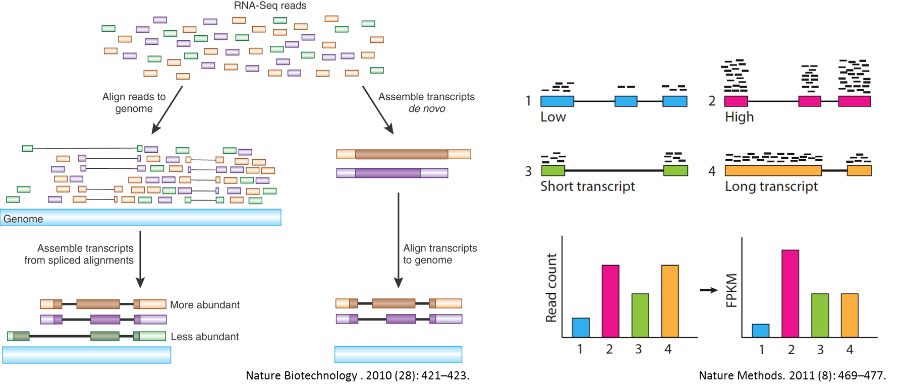
\includegraphics[width=0.9\textwidth]{c3_transcriptome/workflow_bx_02.png}
  \end{figure}
\end{frame}

\begin{frame}
  \frametitle{转录组学 | RNA-Seq | 分析 | 流程 | \textcolor{red}{生信}}
  \begin{figure}
    \centering
    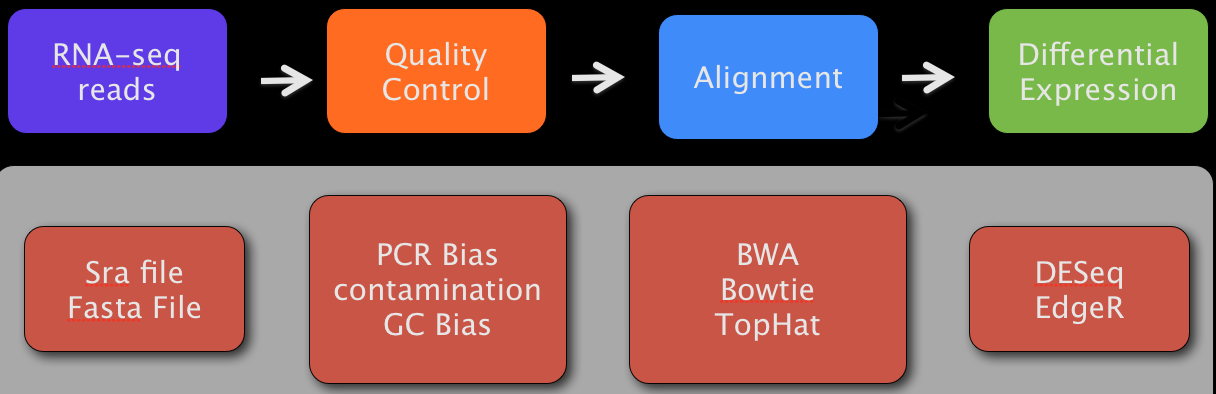
\includegraphics[width=0.7\textwidth]{c3_transcriptome/workflow_bx_03.png}\\
    \vspace{1em}
    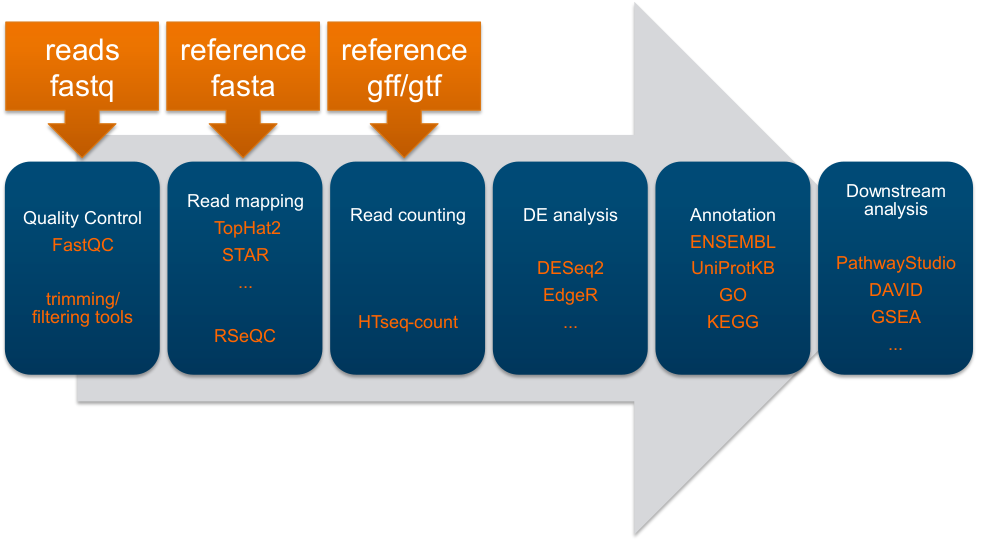
\includegraphics[width=0.7\textwidth]{c3_transcriptome/workflow_bx_30.png}
  \end{figure}
\end{frame}

\begin{frame}
  \frametitle{转录组学 | RNA-Seq | 分析 | 流程 | 生信}
  \begin{figure}
    \centering
    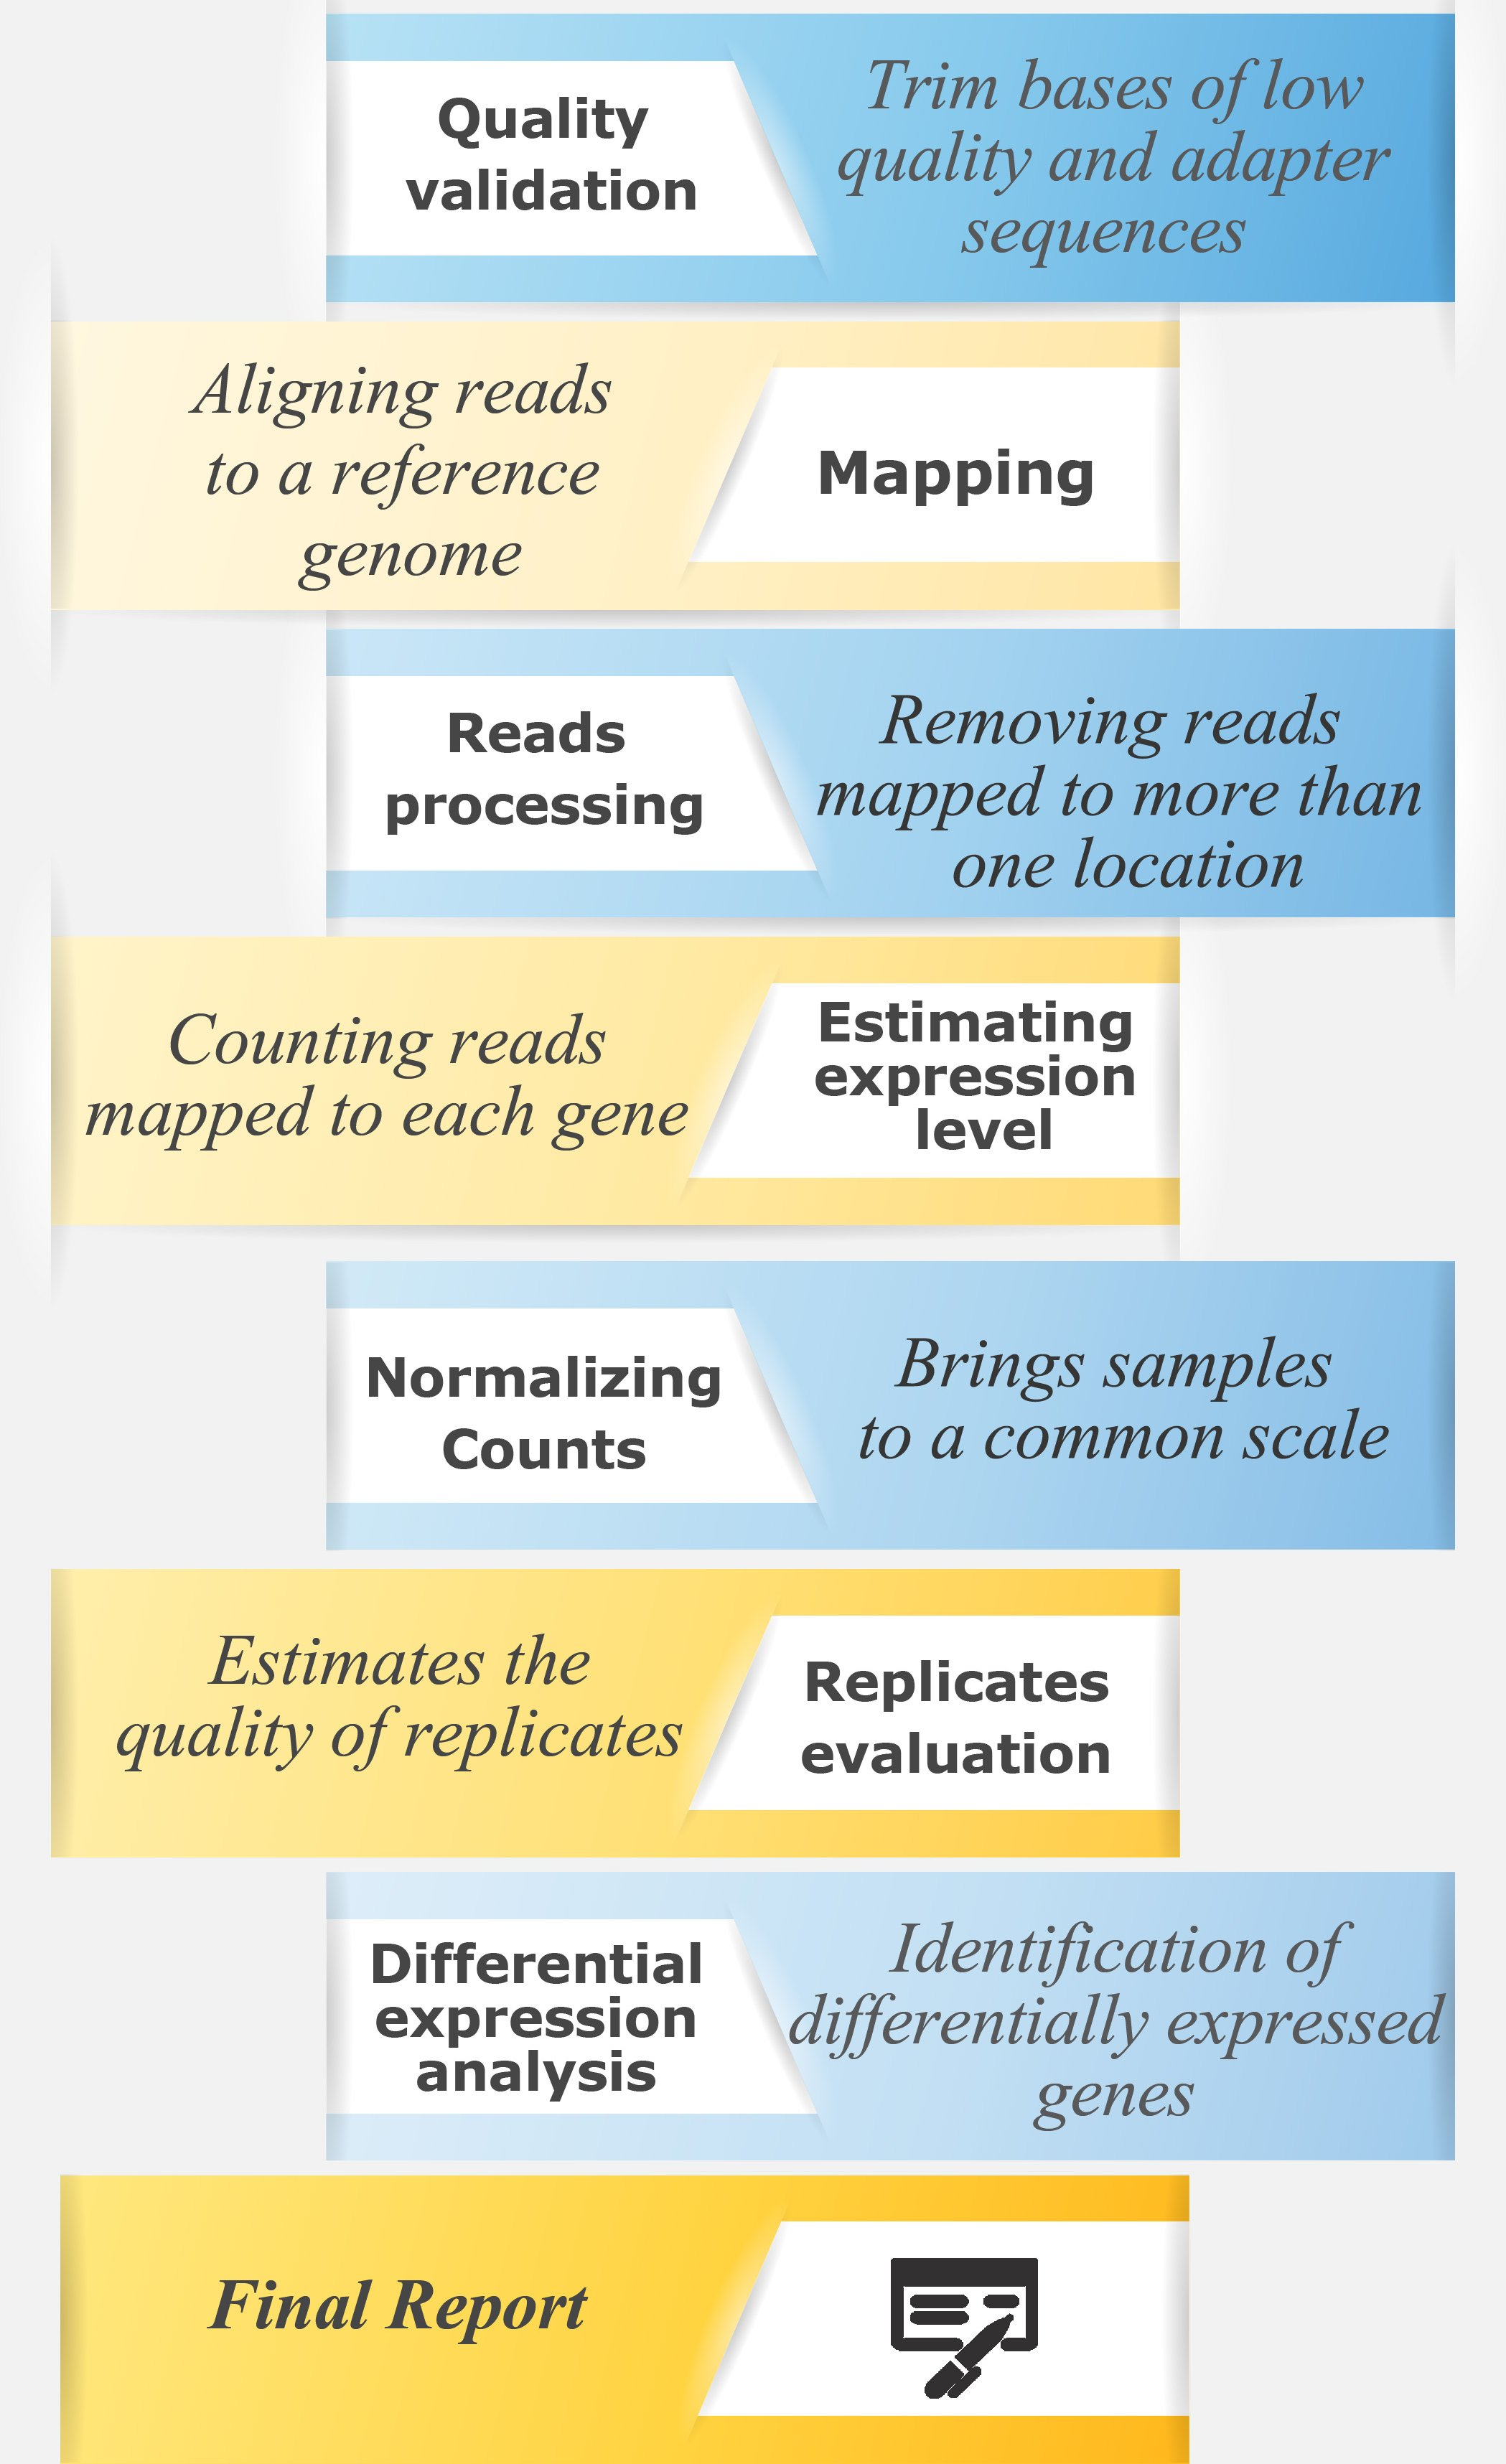
\includegraphics[width=0.4\textwidth]{c3_transcriptome/workflow_bx_04.jpg}
  \end{figure}
\end{frame}

\begin{frame}
  \frametitle{转录组学 | RNA-Seq | 分析 | 流程 | \textcolor{red}{生信}}
  \begin{figure}
    \centering
    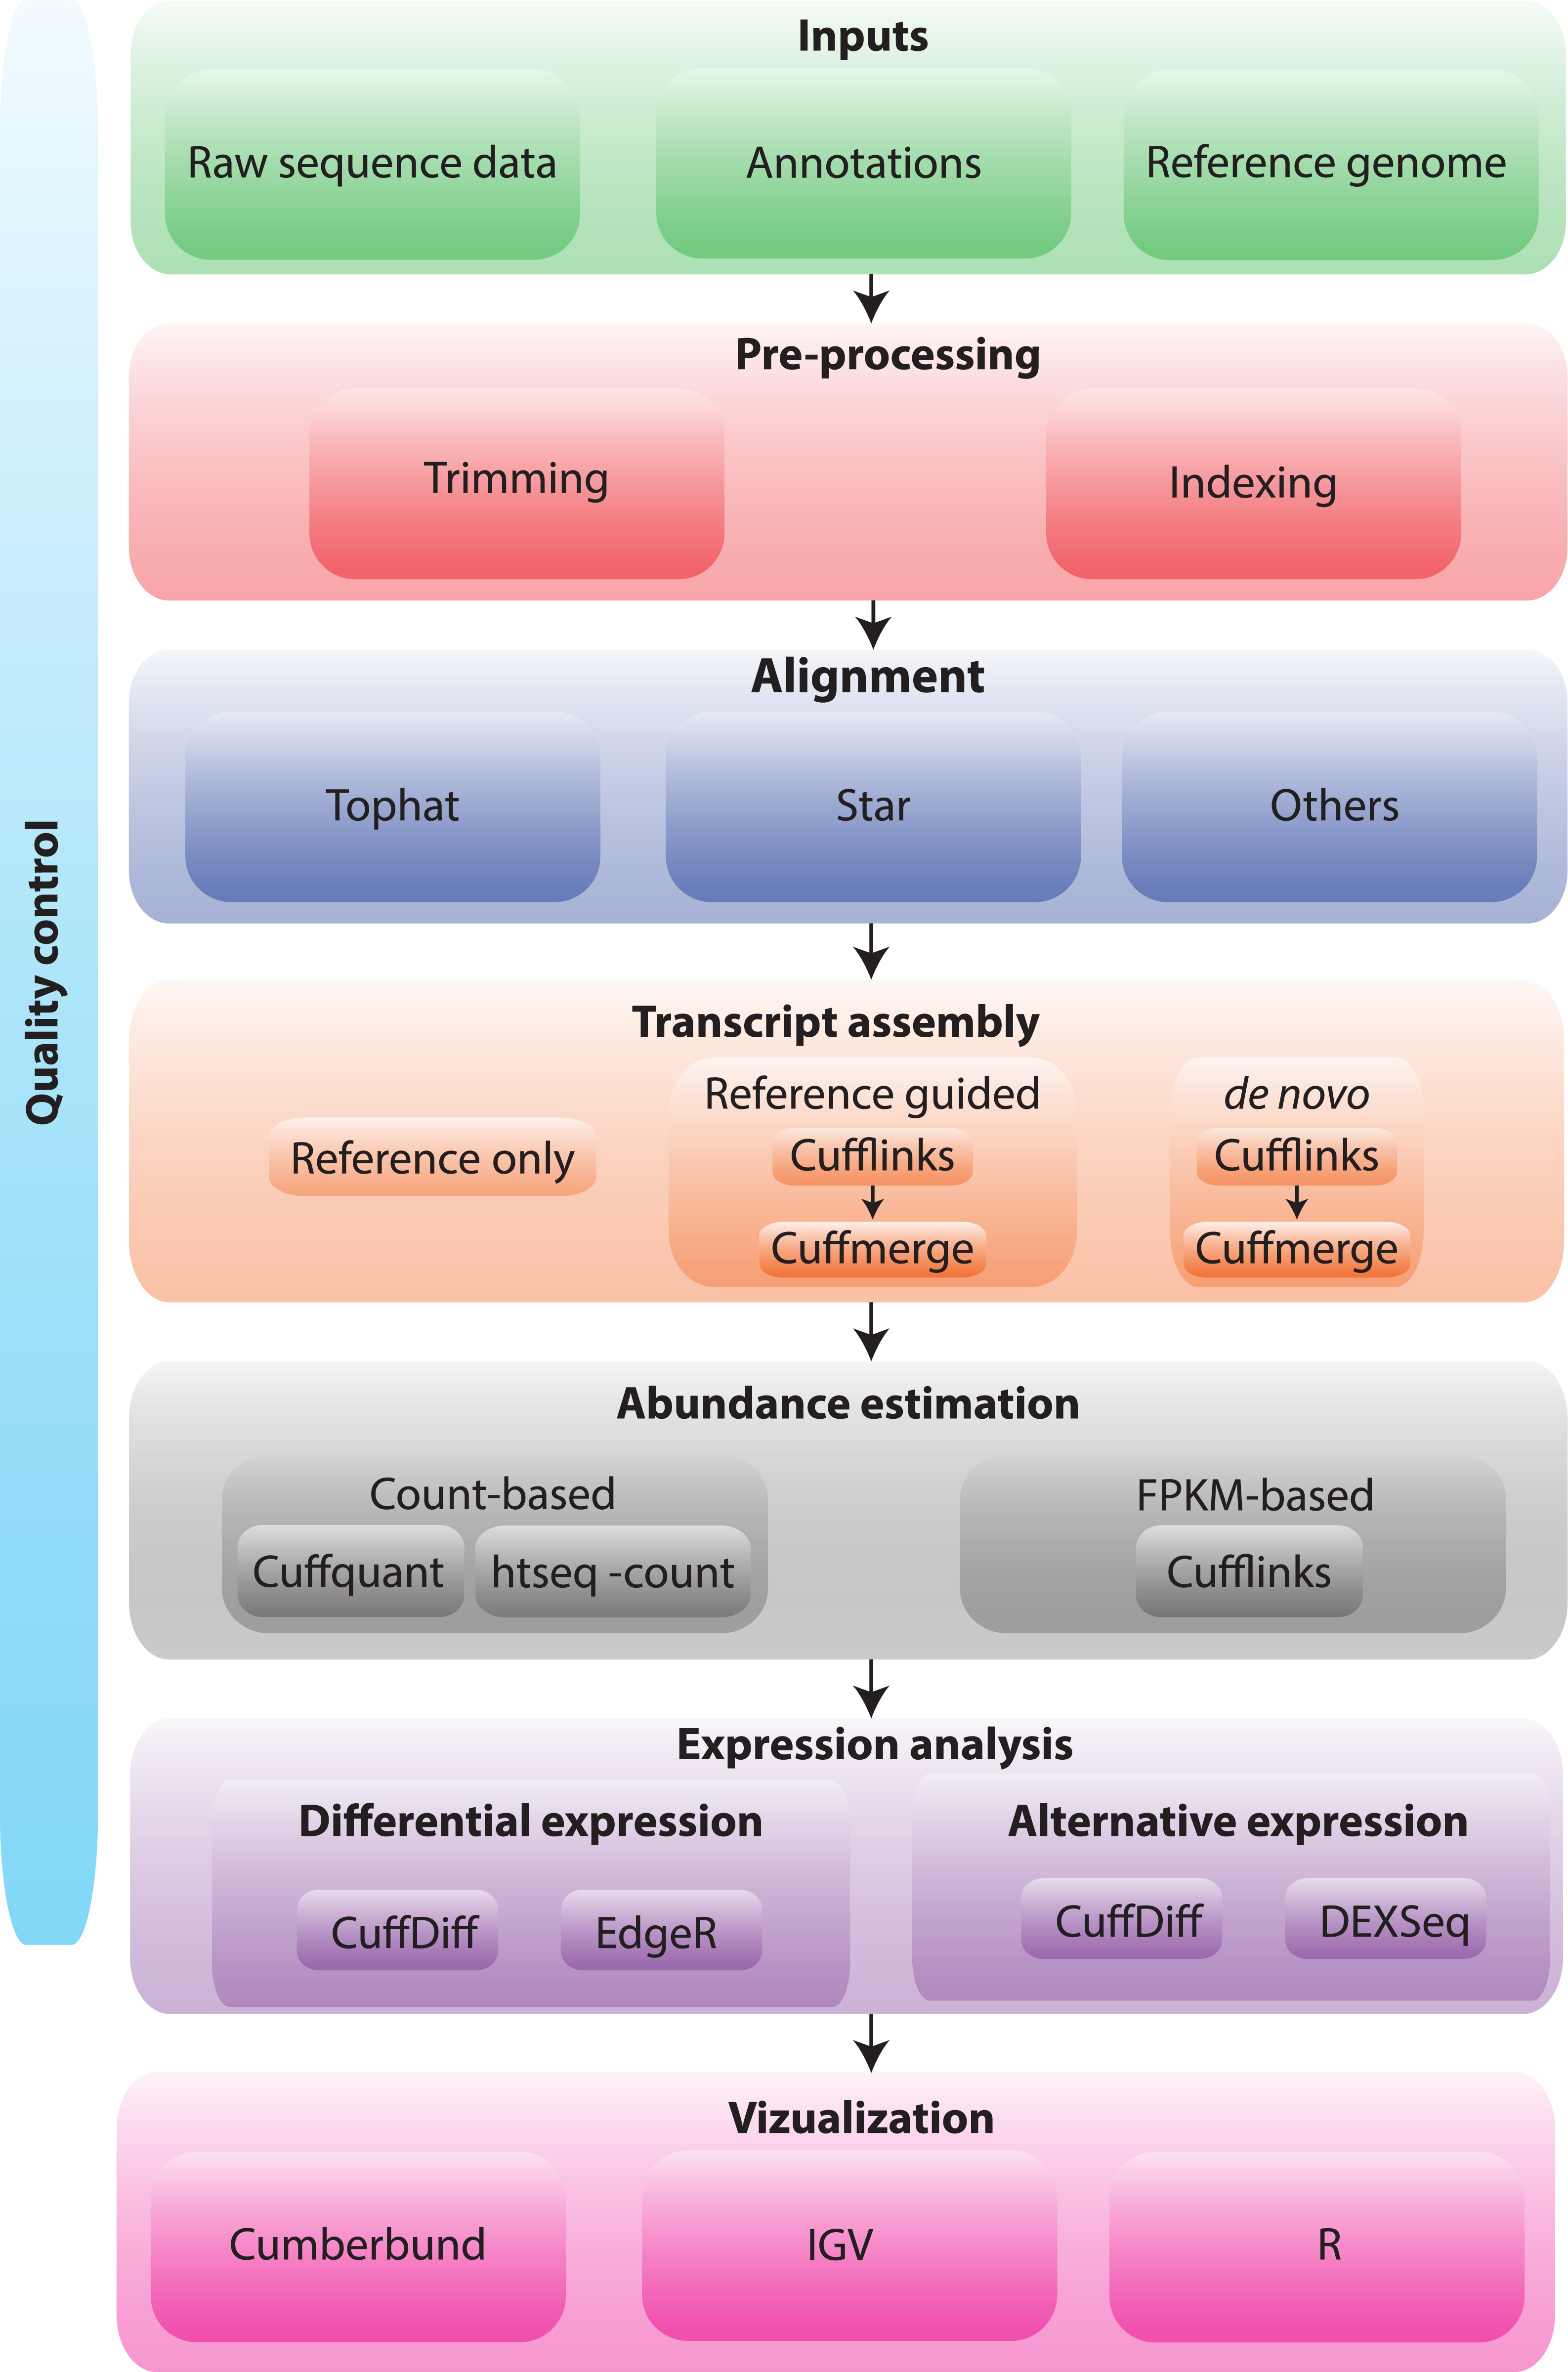
\includegraphics[width=0.4\textwidth]{c3_transcriptome/workflow_bx_05.png}
  \end{figure}
\end{frame}

\begin{frame}
  \frametitle{转录组学 | RNA-Seq | 分析 | 流程 | 补遗 | Single cell}
  \begin{figure}
    \centering
    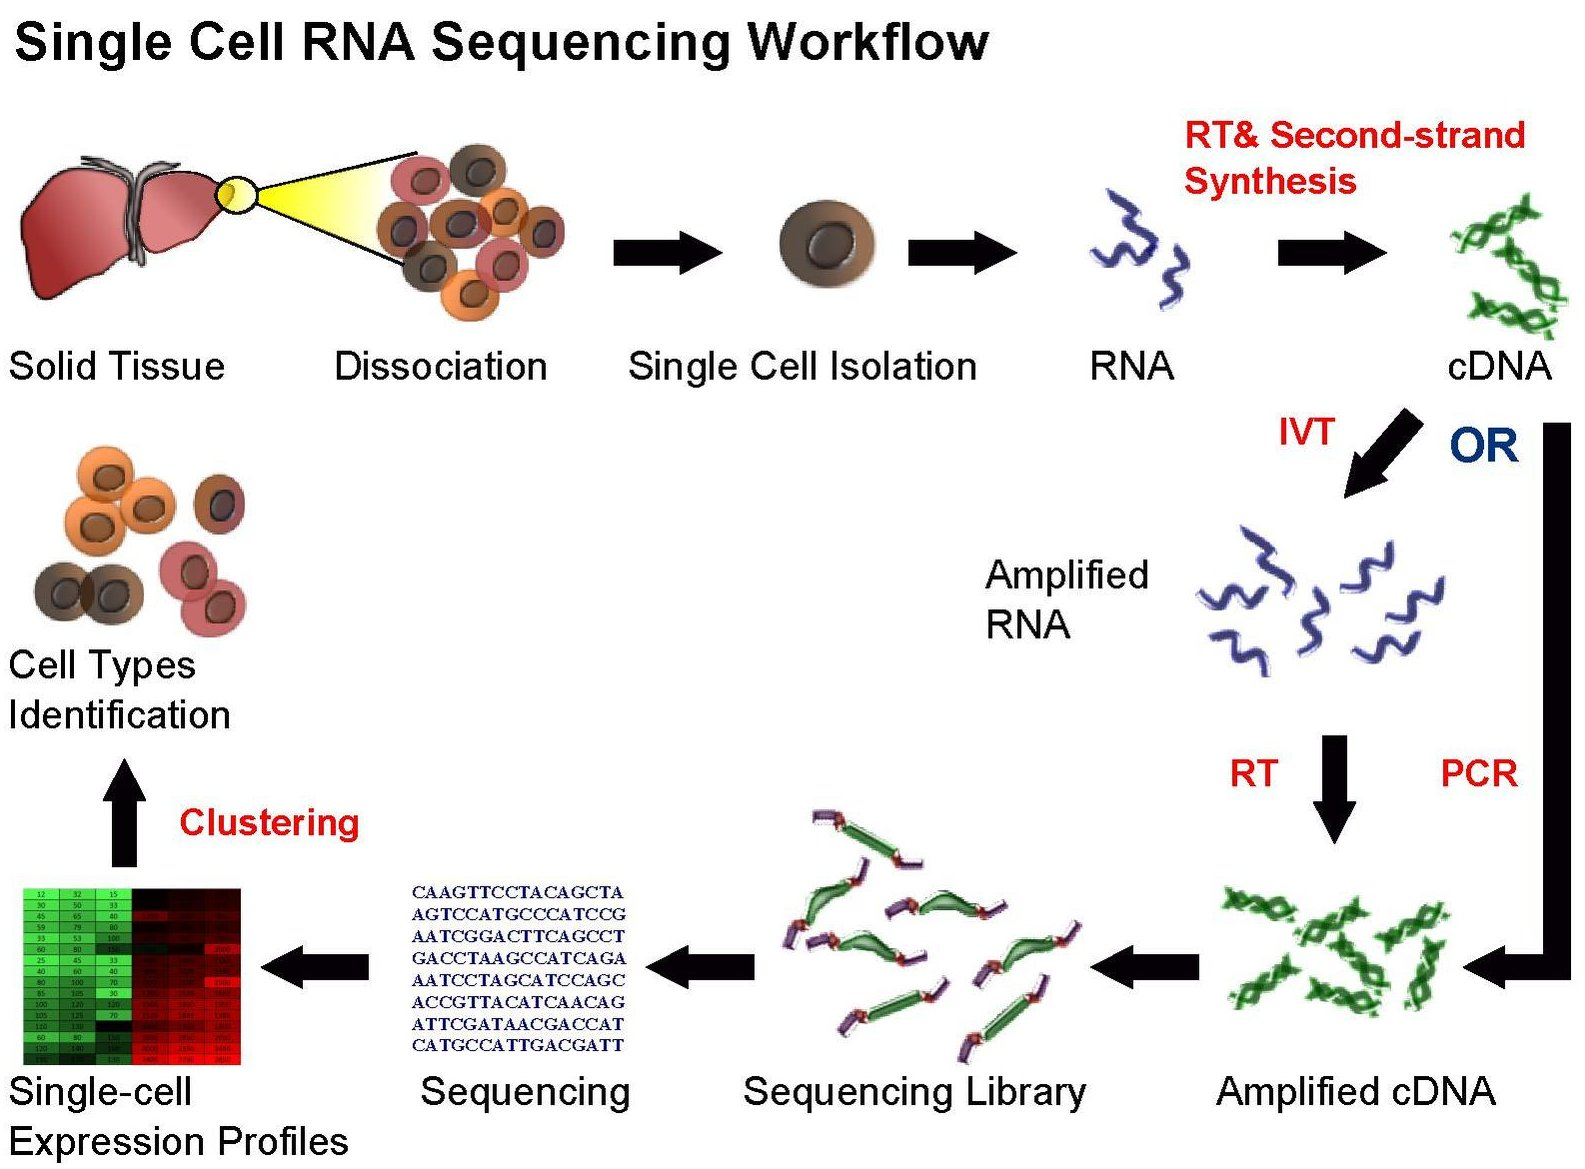
\includegraphics[width=0.85\textwidth]{c3_transcriptome/workflow_single_cell_01.jpg}
  \end{figure}
\end{frame}

\begin{frame}
  \frametitle{转录组学 | RNA-Seq | 分析 | 流程 | 补遗 | Stranded}
  \begin{figure}
    \centering
    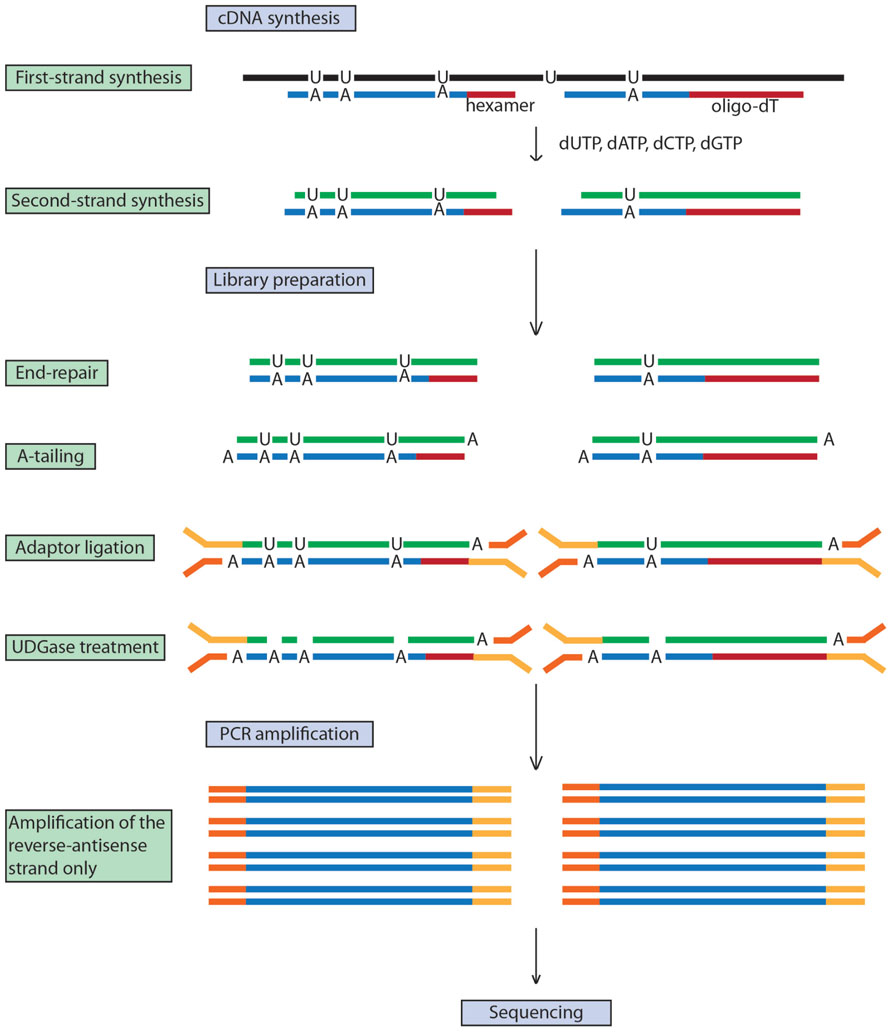
\includegraphics[width=0.55\textwidth]{c3_transcriptome/workflow_strand_01.jpg}
  \end{figure}
\end{frame}

\begin{frame}
  \frametitle{转录组学 | RNA-Seq | 分析 | 流程 | 补遗 | miRNA}
  \begin{figure}
    \centering
    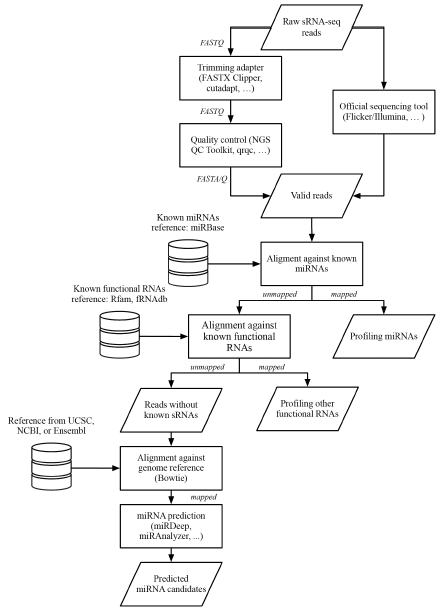
\includegraphics[width=0.48\textwidth]{c3_transcriptome/workflow_mirna_03.png}
  \end{figure}
\end{frame}

\subsubsection{术语}
\begin{frame}
  \frametitle{转录组学 | RNA-Seq | 分析 | 术语 | 引言}
  \begin{figure}
    \centering
    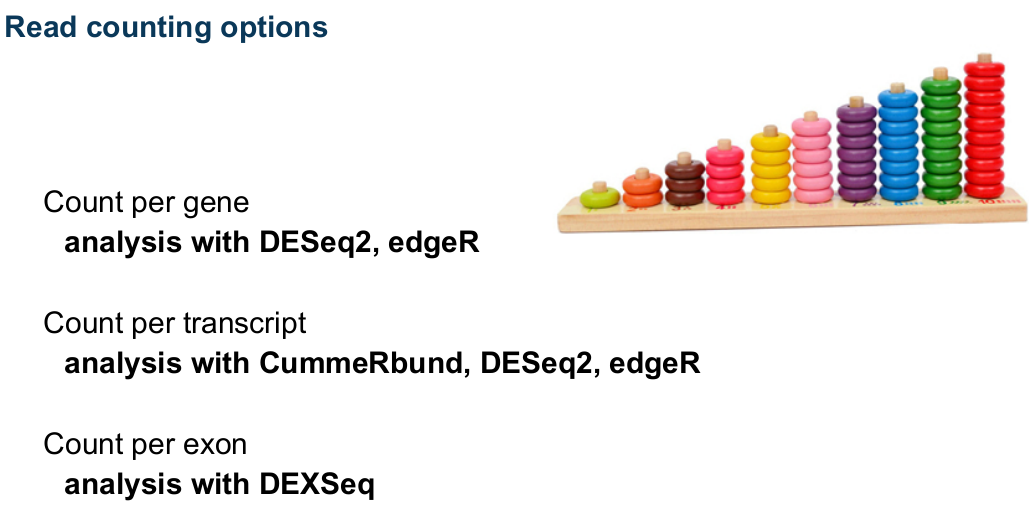
\includegraphics[width=0.9\textwidth]{c3_transcriptome/term_count_01.png}
  \end{figure}
\end{frame}

\begin{frame}
  \frametitle{转录组学 | RNA-Seq | 分析 | 术语 | 引言}
  \begin{figure}
    \centering
    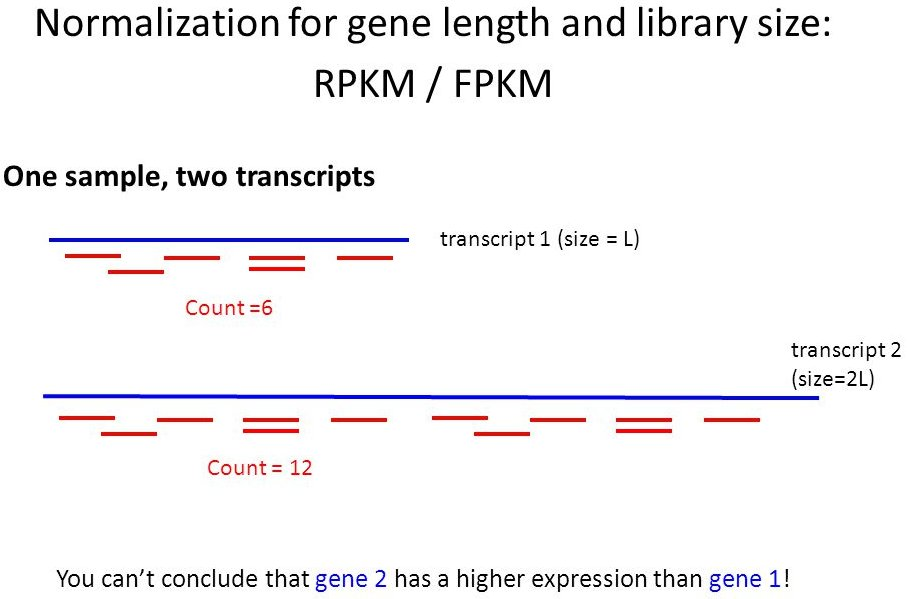
\includegraphics[width=0.9\textwidth]{c3_transcriptome/term_all_01.jpg}
  \end{figure}
\end{frame}

\begin{frame}
  \frametitle{转录组学 | RNA-Seq | 分析 | 术语 | 引言}
  \begin{figure}
    \centering
    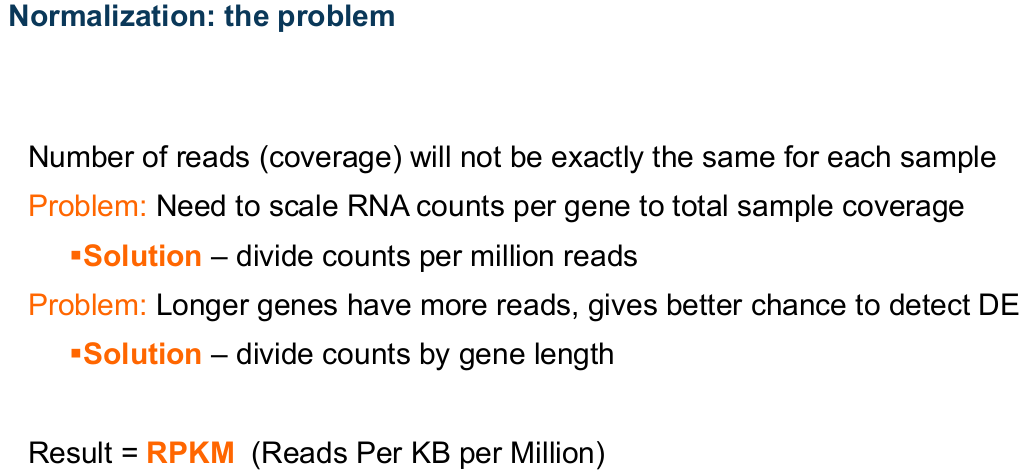
\includegraphics[width=0.9\textwidth]{c3_transcriptome/term_norm_02.png}
  \end{figure}
\end{frame}

\begin{frame}
  \frametitle{转录组学 | RNA-Seq | 分析 | 术语 | 引言}
  \begin{figure}
    \centering
    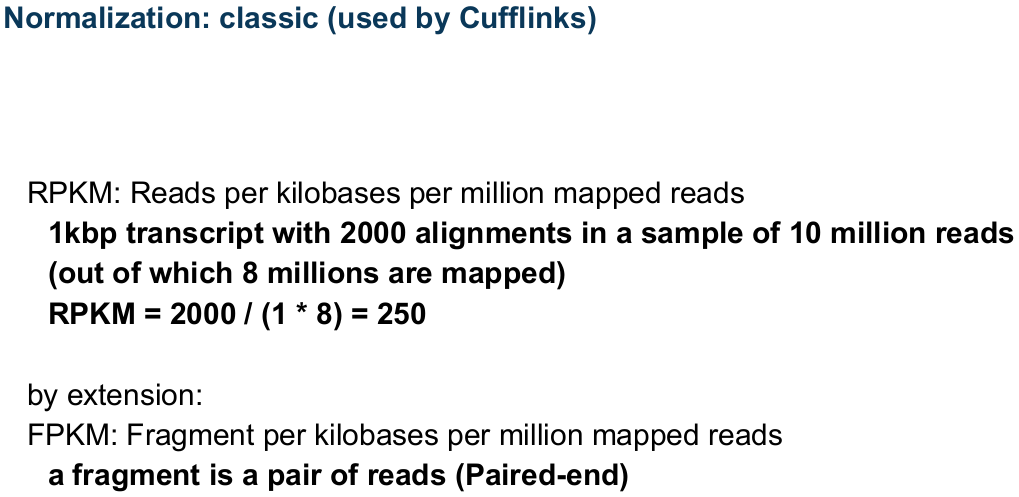
\includegraphics[width=0.9\textwidth]{c3_transcriptome/term_norm_03.png}
  \end{figure}
\end{frame}

\begin{frame}
  \frametitle{转录组学 | RNA-Seq | 分析 | 术语 | 引言}
  \begin{figure}
    \centering
    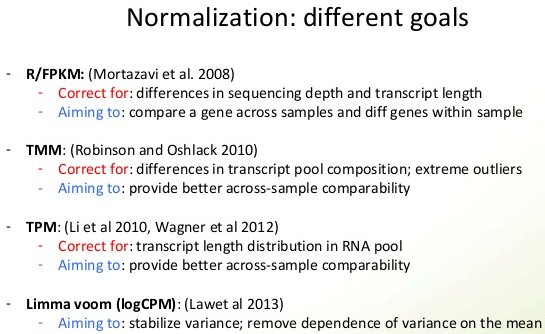
\includegraphics[width=0.9\textwidth]{c3_transcriptome/term_all_02.jpg}
  \end{figure}
\end{frame}

\begin{frame}
  \frametitle{转录组学 | RNA-Seq | 分析 | 术语 | 引言}
  \begin{figure}
    \centering
    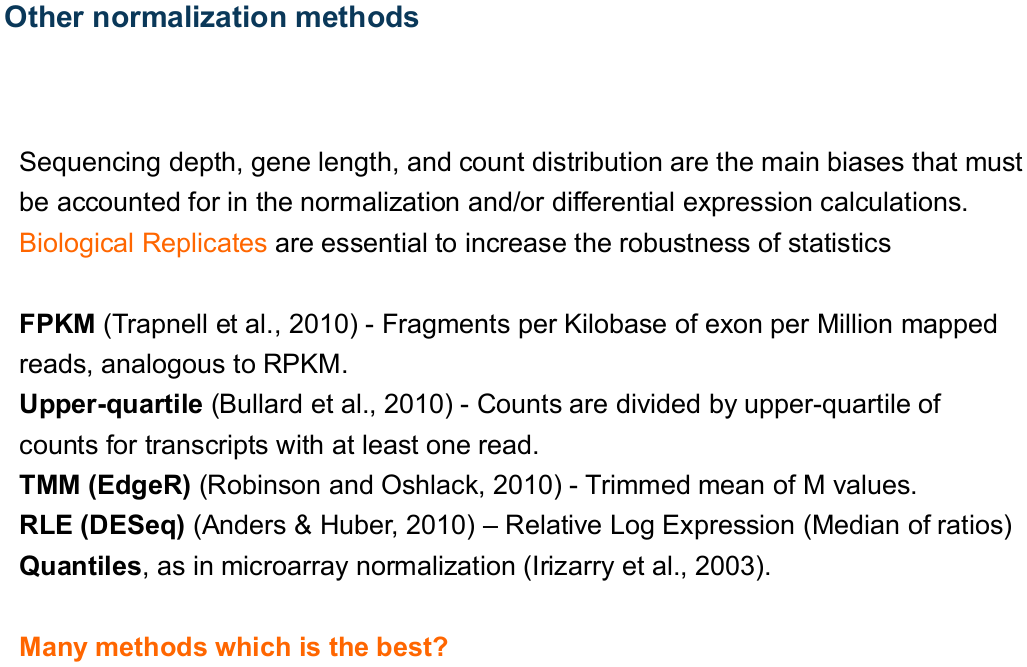
\includegraphics[width=0.9\textwidth]{c3_transcriptome/term_norm_04.png}
  \end{figure}
\end{frame}

\begin{frame}
  \frametitle{转录组学 | RNA-Seq | 分析 | 术语 | 引言}
  \begin{figure}
    \centering
    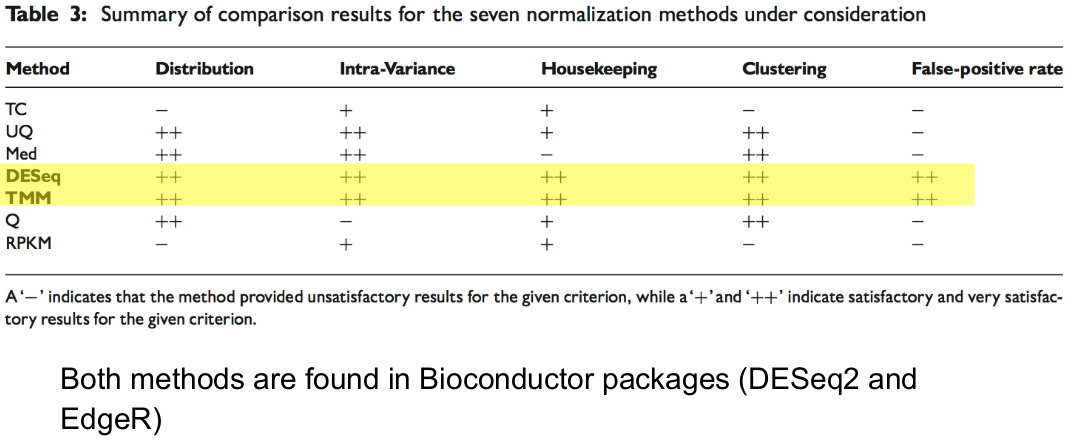
\includegraphics[width=\textwidth]{c3_transcriptome/term_norm_06.png}
  \end{figure}
\end{frame}

\begin{frame}
  \frametitle{转录组学 | RNA-Seq | 分析 | 术语 | \textcolor{red}{引言}}
  \begin{figure}
    \centering
    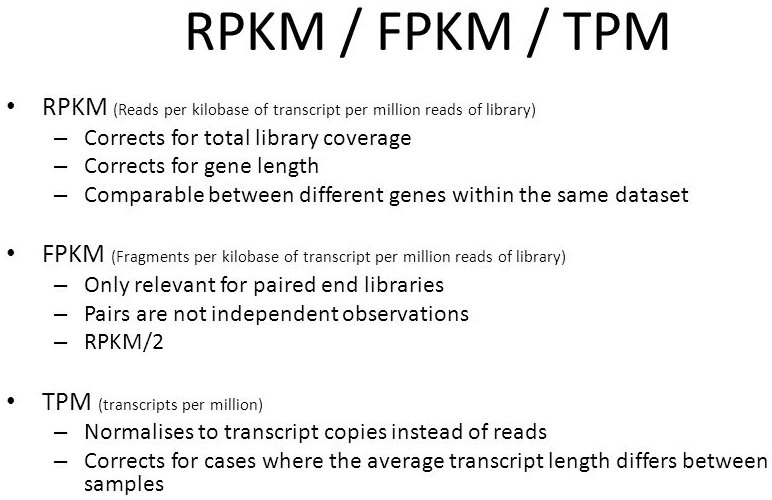
\includegraphics[width=0.9\textwidth]{c3_transcriptome/term_all_04.jpg}
  \end{figure}
\end{frame}

\begin{frame}
  \frametitle{转录组学 | RNA-Seq | 分析 | 术语 | \textcolor{red}{RPKM}}
  \begin{figure}
    \centering
    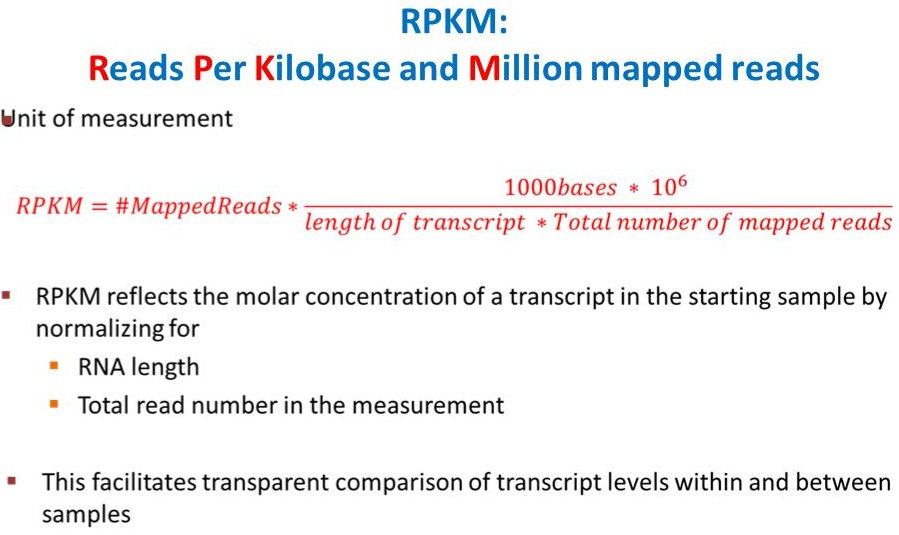
\includegraphics[width=0.8\textwidth]{c3_transcriptome/term_rpkm_01.jpg}\\
    \vspace{1em}
    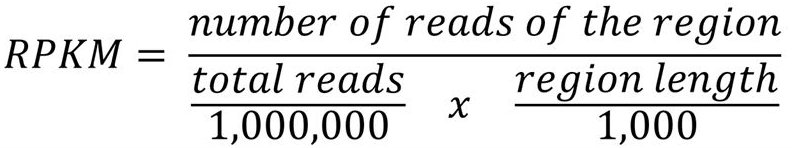
\includegraphics[width=0.7\textwidth]{c3_transcriptome/term_rpkm_02.jpg}
  \end{figure}
\end{frame}

\begin{frame}
  \frametitle{转录组学 | RNA-Seq | 分析 | 术语 | \textcolor{red}{RPKM}}
  \begin{figure}
    \centering
    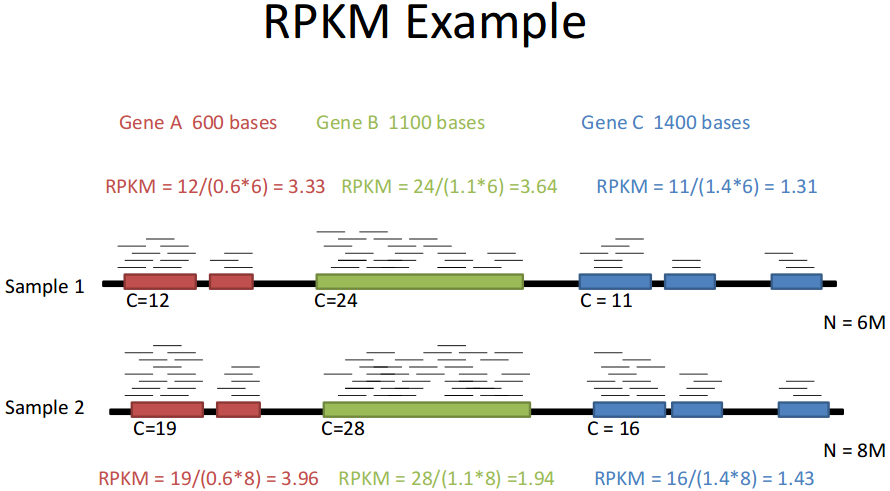
\includegraphics[width=0.9\textwidth]{c3_transcriptome/term_rpkm_03.png}
  \end{figure}
\end{frame}

\begin{frame}
  \frametitle{转录组学 | RNA-Seq | 分析 | 术语 | \textcolor{red}{FPKM}}
  \begin{figure}
    \centering
    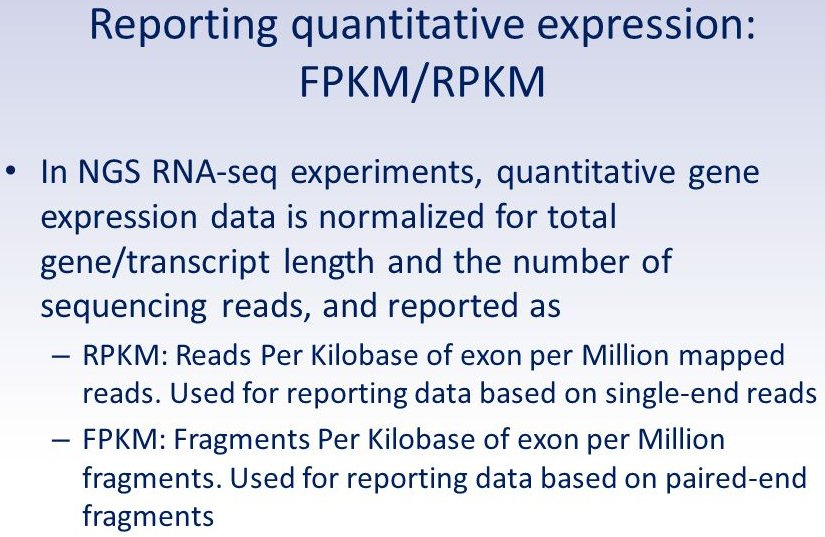
\includegraphics[width=0.9\textwidth]{c3_transcriptome/term_fpkm_01.jpg}
  \end{figure}
\end{frame}

\begin{frame}
  \frametitle{转录组学 | RNA-Seq | 分析 | 术语 | \textcolor{red}{FPKM}}
  \begin{figure}
    \centering
    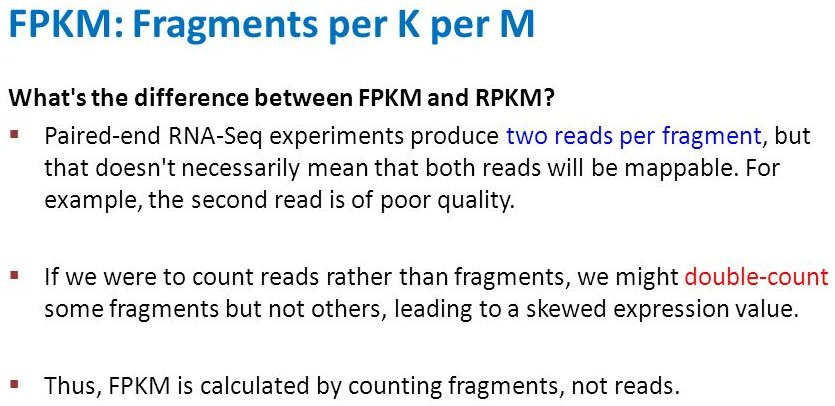
\includegraphics[width=0.8\textwidth]{c3_transcriptome/term_fpkm_02.jpg}\\
    \vspace{1em}
    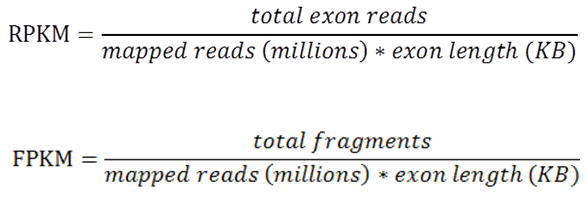
\includegraphics[width=0.6\textwidth]{c3_transcriptome/term_fpkm_03.png}
  \end{figure}
\end{frame}

\begin{frame}
  \frametitle{转录组学 | RNA-Seq | 分析 | 术语 | TPM}
  \begin{block}{TPM}
    当我们进行RNA-Seq时,会使用RPKM或者FPKM来代表某个gene或是isoform的表达量多寡。可是当我们想要比较不同次实验内的某个基因,其表达量相比于“整体基因表达”而言,是否维持在“固定比例”时,便无法使用这样的计算方式。因此Wagner \textit{et. al.}在2012年的时候提出TPM(Transcript Per Million)的概念来弥补这个缺点。
  \end{block}
\end{frame}

\begin{frame}
  \frametitle{转录组学 | RNA-Seq | 分析 | 术语 | \alert{TPM}}
  \begin{figure}
    \centering
    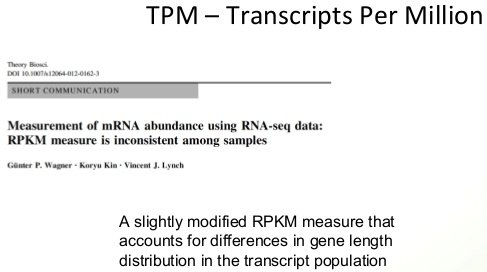
\includegraphics[width=0.7\textwidth]{c3_transcriptome/term_tpm_01.jpg}\\
    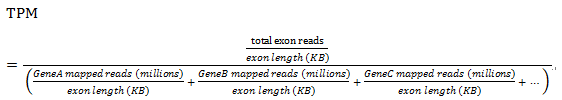
\includegraphics[width=0.7\textwidth]{c3_transcriptome/term_tpm_02.png}\\
    \includegraphics[width=0.3\textwidth]{c3_transcriptome/term_tpm_03.png}
  \end{figure}
\end{frame}

\begin{frame}
  \frametitle{转录组学 | RNA-Seq | 分析 | 术语 | \textcolor{red}{总结}}
  \begin{block}{Metrics}
    \begin{itemize}
      \item RPKM (Reads Per Kilobase Million)
      \item FPKM (Fragments Per Kilobase Million)
      \item TPM (Transcripts Per Kilobase Million)
    \end{itemize}
        These three metrics attempt to normalize for sequencing depth and gene length. 
  \end{block}
\end{frame}

\begin{frame}
  \frametitle{转录组学 | RNA-Seq | 分析 | 术语 | 总结}
  \begin{block}{RPKM}
    Here's how you do it for RPKM:
    \begin{enumerate}
      \item Count up the total reads in a sample and divide that number by 1,000,000 –\ this is our ``per million" scaling factor.
      \item Divide the read counts by the ``per million" scaling factor. This normalizes for sequencing depth, giving you reads per million (RPM)
      \item Divide the RPM values by the length of the gene, in kilobases. This gives you RPKM.
    \end{enumerate}
  \end{block}
\end{frame}

\begin{frame}
  \frametitle{转录组学 | RNA-Seq | 分析 | 术语 | 总结}
  \begin{block}{FPKM}
 FPKM is very similar to RPKM. RPKM was made for single-end RNA-seq, where every read corresponded to a single fragment that was sequenced. FPKM was made for paired-end RNA-seq. With paired-end RNA-seq, two reads can correspond to a single fragment, or, if one read in the pair did not map, one read can correspond to a single fragment. The only difference between RPKM and FPKM is that FPKM takes into account that two reads can map to one fragment (and so it doesn't count this fragment twice). 
  \end{block}
\end{frame}

\begin{frame}
  \frametitle{转录组学 | RNA-Seq | 分析 | 术语 | 总结}
  \begin{block}{TPM}
    TPM is very similar to RPKM and FPKM. The only difference is the order of operations. Here's how you calculate TPM:
    \begin{enumerate}
      \item Divide the read counts by the length of each gene in kilobases. This gives you reads per kilobase (RPK).
      \item Count up all the RPK values in a sample and divide this number by 1,000,000. This is your ``per million" scaling factor.
      \item Divide the RPK values by the ``per million" scaling factor. This gives you TPM.
    \end{enumerate}
    So you see, when calculating TPM, the only difference is that you normalize for gene length first, and then normalize for sequencing depth second. However, the effects of this difference are quite profound.
  \end{block}
\end{frame}

\begin{frame}
  \frametitle{转录组学 | RNA-Seq | 分析 | 术语 | 总结}
  {\footnotesize
  \begin{block}{Compare}
    When you use TPM, the sum of all TPMs in each sample are the same. This makes it easier to compare the proportion of reads that mapped to a gene in each sample. In contrast, with RPKM and FPKM, the sum of the normalized reads in each sample may be different, and this makes it harder to compare samples directly.\\
    \vspace{0.5em}
    Here's an example. If the TPM for gene A in Sample 1 is 3.33 and the TPM in sample B is 3.33, then I know that the exact same proportion of total reads mapped to gene A in both samples. This is because the sum of the TPMs in both samples always add up to the same number (so the denominator required to calculate the proportions is the same, regardless of what sample you are looking at.)\\
    \vspace{0.5em}
    With RPKM or FPKM, the sum of normalized reads in each sample can be different. Thus, if the RPKM for gene A in Sample 1 is 3.33 and the RPKM in Sample 2 is 3.33, I would not know if the same proportion of reads in Sample 1 mapped to gene A as in Sample 2. This is because the denominator required to calculate the proportion could be different for the two samples.
  \end{block}
  }
\end{frame}

\subsubsection{分析}
\begin{frame}
  \frametitle{转录组学 | RNA-Seq | 分析 | 工具 | \textcolor{red}{概览}}
  \begin{figure}
    \centering
    \includegraphics[width=0.75\textwidth]{c3_transcriptome/tool_pipeline_01.jpg}
  \end{figure}
\end{frame}

\begin{frame}
  \frametitle{转录组学 | RNA-Seq | 分析 | 工具 | \textcolor{red}{Quality control}}
  \begin{block}{Quality control}
    \begin{itemize}
      \item FastQC: FastQC is a quality control tool for high-throughput sequence data (Babraham Institute) and is developed in Java. Import of data is possible from FastQ files, BAM or SAM format. This tool provides an overview to inform about problematic areas, summary graphs and tables to rapid assessment of data. Results are presented in HTML permanent reports. FastQC can be run as a stand-alone application or it can be integrated into a larger pipeline solution.
      \item NGSQC: cross-platform quality analysis pipeline for deep sequencing data.
    \end{itemize}
  \end{block}
\end{frame}

\begin{frame}
  \frametitle{转录组学 | RNA-Seq | 分析 | 工具 | \textcolor{red}{Quality control}}
  {\footnotesize
  \begin{block}{Quality control}
    \begin{itemize}
      \item RNA-SeQC: RNA-SeQC is a tool with application in experiment design, process optimization and quality control before computational analysis. Essentially, provides three types of quality control: read counts (such as duplicate reads, mapped reads and mapped unique reads, rRNA reads, transcript-annotated reads, strand specificity), coverage (like mean coverage, mean coefficient of variation, 5'/3' coverage, gaps in coverage, GC bias) and expression correlation (the tool provides RPKM-based estimation of expression levels). RNA-SeQC is implemented in Java and is not required installation, however can be run using the GenePattern web interface. The input could be one or more BAM files. HTML reports are generated as output.
      \item RSeQC: RSeQC analyzes diverse aspects of RNA-Seq experiments: sequence quality, sequencing depth, strand specificity, GC bias, read distribution over the genome structure and coverage uniformity. The input can be SAM, BAM, FASTA, BED files or Chromosome size file (two-column, plain text file). Visualization can be performed by genome browsers like UCSC, IGB and IGV. However, R scripts can also be used to visualization.
    \end{itemize}
  \end{block}
  }
\end{frame}

\begin{frame}
  \frametitle{转录组学 | RNA-Seq | 分析 | 工具 | \textcolor{red}{Trimming and adapters removal}}
    {\footnotesize
  \begin{block}{Trimming and adapters removal}
    \begin{itemize}
      \item FASTX: FASTX Toolkit is a set of command line tools to manipulate reads in files FASTA or FASTQ format. These commands make possible preprocess the files before mapping with tools like Bowtie. Some of the tasks allowed are: conversion from FASTQ to FASTA format, information about statistics of quality, removing sequencing adapters, filtering and cutting sequences based on quality or conversion DNA/RNA.
      \item PRINSEQ: PRINSEQ generates statistics of your sequence data for sequence length, GC content, quality scores, n-plicates, complexity, tag sequences, poly-A/T tails, odds ratios. Filter the data, reformat and trim sequences.
      \item cutadapt: Cutadapt finds and removes adapter sequences, primers, poly-A tails and other types of unwanted sequence from your high-throughput sequencing reads.
    \end{itemize}
  \end{block}
  }
\end{frame}

\begin{frame}
  \frametitle{转录组学 | RNA-Seq | 分析 | 工具 | Alignment}
  \begin{figure}
    \centering
    \includegraphics[width=0.7\textwidth]{c3_transcriptome/tool_alignment_01.png}
  \end{figure}
\end{frame}

\begin{frame}
  \frametitle{转录组学 | RNA-Seq | 分析 | 工具 | \textcolor{red}{Alignment}}
  \begin{block}{\textit{De novo} Splice Aligners that also use annotation optionally}
    TopHat: TopHat is prepared to find \textit{de novo} junctions. TopHat aligns reads in two steps. Firstly, unspliced reads are aligned with Bowtie. After, the aligned reads are assembled with Maq resulting islands of sequences. Secondly, the splice junctions are determined based on the initially unmapped reads and the possible canonical donor and acceptor sites within the island sequences.
  \end{block}
  \pause
  \begin{block}{graph-based alignment of next generation sequencing reads to a population of genomes}
    HISAT2: HISAT2 is a fast and sensitive alignment program for mapping next-generation sequencing reads (both DNA and RNA) to a population of human genomes (as well as to a single reference genome).
  \end{block}
\end{frame}

\begin{frame}
  \frametitle{转录组学 | RNA-Seq | 分析 | 工具 | \textcolor{red}{Transcriptome assemblers}}
  \begin{block}{Genome-Guided assemblers}
    \begin{itemize}
      \item Cufflinks: Cufflinks assembles transcripts, estimates their abundances, and tests for differential expression and regulation in RNA-Seq samples. It accepts aligned RNA-Seq reads and assembles the alignments into a parsimonious set of transcripts. Cufflinks then estimates the relative abundances of these transcripts based on how many reads support each one, taking into account biases in library preparation protocols.
      \item Scripture: Scripture is a method for transcriptome reconstruction that relies solely on RNA-Seq reads and an assembled genome to build a transcriptome \textit{ab initio}. The statistical methods to estimate read coverage significance are also applicable to other sequencing data. Scripture also has modules for ChIP-Seq peak calling.
    \end{itemize}
  \end{block}
\end{frame}

\begin{frame}
  \frametitle{转录组学 | RNA-Seq | 分析 | 工具 | \textcolor{red}{Expression}}
  {\footnotesize
  \begin{block}{Normalization, Quantitative analysis and Differential Expression}
    \begin{itemize}
      \item Cufflinks/Cuffdiff: Cufflinks is appropriate to measure global \textit{de novo} transcript isoform expression. It performs assembly of transcripts, estimation of abundances and determines differential expression (Cuffdiff) and regulation in RNA-Seq samples.
      \item DESeq: DESeq is a Bioconductor package to perform differential gene expression analysis based on negative binomial distribution.
      \item EdgeR: EdgeR is a R package for analysis of differential expression of data from DNA sequencing methods, like RNA-Seq, SAGE or ChIP-Seq data. edgeR employs statistical methods supported on negative binomial distribution as a model for count variability.
      \item DEGseq: DEGseq is an R package to identify differentially expressed genes from RNA-Seq data.
      \item baySeq: This package identifies differential expression in high-throughput `count' data, such as that derived from next-generation sequencing machines, calculating estimated posterior likelihoods of differential expression (or more complex hypotheses) via empirical Bayesian methods.
    \end{itemize}
  \end{block}
}
\end{frame}

\begin{frame}
  \frametitle{转录组学 | RNA-Seq | 分析 | 工具 | \textcolor{red}{Workbench}}
  {\footnotesize
  \begin{block}{Analysis pipeline/Integrated solutions}
    \begin{itemize}
      \item easyRNASeq: easyRNASeq calculates the coverage of high-throughput short-reads against a genome of reference and summarizes it per feature of interest (e.g. exon, gene, transcript). The data can be normalized as `RPKM' or by the `DESeq' or `edgeR' package.
      \item Galaxy: Galaxy is a general purpose workbench platform for computational biology. There are several publicly accessible Galaxy servers that support RNA-Seq tools and workflows, including NBIC's Andromeda, the CBIIT-Giga server, the Galaxy Project's public server, the GeneNetwork Galaxy server, the University of Oslo's Genomic Hyperbrowser, URGI's server (which supports S-MART), and many others.
      \item GenePattern: GenePattern offers integrated solutions to RNA-Seq analysis.
      \item Taverna: Taverna is an open source and domain-independent Workflow Management System – a suite of tools used to design and execute scientific workflows and aid \textit{in silico} experimentation.
    \end{itemize}
  \end{block}
  }
\end{frame}

\begin{frame}
  \frametitle{转录组学 | RNA-Seq | 分析 | 工具 | \textcolor{red}{Framework}}
  {\footnotesize
  \begin{block}{RNACocktail}
The RNACocktail pipeline is composed of a high-accuracy tools for different steps of RNA-Seq analysis. It performs a broad spectrum RNA-Seq analysis on both short- and long-read technologies to enable meaningful insights from transcriptomic data. It was developed after analyzing a variety of RNA-Seq samples (ranging from germline, cancer to stem cell datasets) and technologies using a multitude of tool combinations to determine a pipeline which is comprehensive, fast and accurate. RNACocktail supports:
  \end{block}
  }
  \vspace{-0.5em}
    \begin{table}
    \centering
    \rowcolors[]{1}{blue!20}{blue!10}
    \begin{tabular}{ll}
      \hline
      \rowcolor{blue!50}short-read & long-read\\
      \hline
      alignment	& error correction\\
      transcriptome reconstruction & alignment\\
      denovo transcriptome assembly	& transcriptome reconstruction\\
      alignment-free quantification	& fusion prediction\\
      differential expression analysis & ---\\
      fusion prediction	& ---\\
      variant calling	& ---\\
      RNA editing prediction & ---\\
      \hline
    \end{tabular}
  \end{table}
\end{frame}

% \begin{frame}
%   \frametitle{转录组学 | RNA-Seq | 分析 | 工具 | Framework | RNACocktail}
%   \begin{figure}
%     \centering
%     \includegraphics[width=0.8\textwidth]{c3_transcriptome/tool_rnacocktail_01.jpg}
%   \end{figure}
% \end{frame}

\begin{frame}
  \frametitle{转录组学 | RNA-Seq | 分析 | 工具 | Framework | RNACocktail}
  \begin{figure}
    \centering
    \includegraphics[width=0.6\textwidth]{c3_transcriptome/tool_rnacocktail_02.jpg}
  \end{figure}
\end{frame}

\begin{frame}
  \frametitle{转录组学 | RNA-Seq | 分析 | 工具 | \textcolor{red}{Visualization}}
  {\footnotesize
  \begin{block}{Visualization tools}
    \begin{itemize}
      \item ngs.plot: Quick mining and visualization of next-generation sequencing data by integrating genomic databases. It allows to easily visualize NGS samples at functional genomic regions.
      \item GBrowse: GBrowse is a combination of database and interactive web pages for manipulating and displaying annotations on genomes.
      \item IGB: The Integrated Genome Browser (IGB, pronounced ig-bee) is an application intended for visualization and exploration of genomes and corresponding annotations from multiple data sources. 
      \item IGV: The Integrative Genomics Viewer (IGV) is a high-performance visualization tool for interactive exploration of large, integrated genomic datasets.
      \item SeqMonk: SeqMonk is a program to enable the visualisation and analysis of mapped sequence data. It was written for use with mapped next generation sequence data but can in theory be used for any dataset which can be expressed as a series of genomic positions.
      \item Tablet: Tablet is a lightweight, high-performance graphical viewer for next generation sequence assemblies and alignments.
    \end{itemize}
  \end{block}
  }
\end{frame}

\begin{frame}
  \frametitle{转录组学 | RNA-Seq | 分析 | 工具 | \textcolor{red}{Databases}}
  \begin{block}{RNA-Seq Databases}
    \begin{itemize}
      \item ENCODE: Encyclopedia of DNA Elements
      \item GTEx: Genotype-Tissue Expression (GTEx) project
      \item RNA-Seq Atlas: A reference database for gene expression profiling in normal tissue by next-generation sequencing.
      \item SRA: The Sequence Read Archive (SRA) stores raw sequence data from ``next-generation" sequencing technologies including 454, IonTorrent, Illumina, SOLiD, Helicos and Complete Genomics. In addition to raw sequence data, SRA now stores alignment information in the form of read placements on a reference sequence.
    \end{itemize}
  \end{block}
\end{frame}

\begin{frame}
  \frametitle{转录组学 | RNA-Seq | 分析 | 工具 | Pipeline | \textcolor{red}{Tuxedo}}
  {\footnotesize
  \begin{block}{Tuxedo}
    The RNA-seq pipeline ``Tuxedo" consists of the \textcolor{red}{TopHat} spliced read mapper, that internally uses \textcolor{red}{Bowtie/Bowtie2} short read aligners, and several \textcolor{red}{Cufflinks} tools that allows one to assemble transcripts, estimate their abundances, and tests for differential expression and regulation in RNA-Seq samples.
  \end{block}
}
  \begin{figure}
    \centering
    \includegraphics[width=0.7\textwidth]{c3_transcriptome/tool_tc_06.png}
  \end{figure}
\end{frame}

\begin{frame}
  \frametitle{转录组学 | RNA-Seq | 分析 | 工具 | Pipeline | \textcolor{red}{Tuxedo}}
  \begin{figure}
    \centering
    \includegraphics[width=0.8\textwidth]{c3_transcriptome/tool_tc_08.png}
  \end{figure}
\end{frame}

\begin{frame}
  \frametitle{转录组学 | RNA-Seq | 分析 | 工具 | Pipeline | \textcolor{red}{Tuxedo}}
  \begin{figure}
    \centering
    \includegraphics[width=0.45\textwidth]{c3_transcriptome/tool_tc_01.png}
  \end{figure}
\end{frame}

\begin{frame}
  \frametitle{转录组学 | RNA-Seq | 分析 | 工具 | Pipeline | \textcolor{red}{Tuxedo}}
  \begin{figure}
    \centering
    \includegraphics[width=0.65\textwidth]{c3_transcriptome/tool_tc_03.png}\\
    \vspace{0.5em}
    \includegraphics[width=0.62\textwidth]{c3_transcriptome/tool_tc_04.png}
  \end{figure}
\end{frame}

\begin{frame}
  \frametitle{转录组学 | RNA-Seq | 分析 | 工具 | Pipeline | \textcolor{red}{Tuxedo}}
  \begin{figure}
    \centering
    \includegraphics[width=0.9\textwidth]{c3_transcriptome/tool_tc_13.png}
  \end{figure}
\end{frame}

\begin{frame}
  \frametitle{转录组学 | RNA-Seq | 分析 | 工具 | Pipeline | \textcolor{red}{Tuxedo}}
  \begin{block}{Bowtie: ultrafast short read alignment}
    Bowtie is an ultrafast and memory-efficient tool for aligning sequencing reads to long reference sequences. It is particularly good at aligning reads of about 50 up to 100s or 1,000s of characters, and particularly good at aligning to relatively long (e.g. mammalian) genomes. Bowtie 2 indexes the genome with an FM Index to keep its memory footprint small: for the human genome, its memory footprint is typically around 3.2 GB. Bowtie 2 supports gapped, local, and paired-end alignment modes.
  \end{block}
  \pause
  \begin{block}{TopHat: alignment of short RNA-Seq reads}
    TopHat is a fast splice junction mapper for RNA-Seq reads. It aligns RNA-Seq reads to mammalian-sized genomes using the ultra high-throughput short read aligner Bowtie, and then analyzes the mapping results to identify splice junctions between exons.
  \end{block}
\end{frame}

\begin{frame}
  \frametitle{转录组学 | RNA-Seq | 分析 | 工具 | Pipeline | \textcolor{red}{Tuxedo}}
  \begin{block}{Cufflinks: transcriptome assembly and differential expression analysis for RNA-Seq}
    Cufflinks assembles transcripts, estimates their abundances, and tests for differential expression and regulation in RNA-Seq samples. It accepts aligned RNA-Seq reads and assembles the alignments into a parsimonious set of transcripts. Cufflinks then estimates the relative abundances of these transcripts based on how many reads support each one, taking into account biases in library preparation protocols.
  \end{block}
  \pause
  \begin{block}{CummeRbund: visualization of RNA-Seq differential analysis}
    CummeRbund is an R package that is designed to aid and simplify the task of analyzing Cufflinks RNA-Seq output.
  \end{block}
\end{frame}

\begin{frame}
  \frametitle{转录组学 | RNA-Seq | 分析 | 工具 | Pipeline | \textcolor{red}{Tuxedo}}
  \begin{block}{Cufflinks}
    Cufflinks is both the name of a suite of tools and a program within that suite. Cufflinks the program assembles transcriptomes from RNA-Seq data and quantifies their expression.
  \end{block}
  \pause
  \begin{block}{Cuffcompare}
    Cuffcompare helps you compare the transcriptomes assembled from different RNA-Seq libraries and assess the quality of your assembly.
  \end{block}
  \pause
  \begin{block}{Cuffmerge}
    Cuffmerge merges the assembled transcriptomes into a master transcriptome. This step is required for a differential expression analysis of the new transcripts you've assembled. 
  \end{block}
\end{frame}

\begin{frame}
  \frametitle{转录组学 | RNA-Seq | 分析 | 工具 | Pipeline | \textcolor{red}{Tuxedo}}
  \begin{block}{Cuffquant}
    Cuffquant computes the gene and transcript expression profiles and save these profiles to files that you can analyze later with Cuffdiff or Cuffnorm. It is recommended for analyses involving more than a handful of libraries.
  \end{block}
  \pause
  \begin{block}{Cuffdiff}
    Cuffdiff is a highly accurate tool for performing the comparisons of expression levels of genes and transcripts.
  \end{block}
  \pause
  \begin{block}{Cuffnorm}
    Cuffnorm normalizes a set of samples to be on as similar scales as possible, which can improve the results you obtain with other downstream tools.
  \end{block}
\end{frame}

\begin{frame}
  \frametitle{转录组学 | RNA-Seq | 分析 | 工具 | Pipeline | Tuxedo}
  \begin{figure}
    \centering
    \includegraphics[width=0.9\textwidth]{c3_transcriptome/tool_tophat_02.png}
  \end{figure}
\end{frame}

\begin{frame}
  \frametitle{转录组学 | RNA-Seq | 分析 | 工具 | Pipeline | Tuxedo}
  \begin{figure}
    \centering
    \includegraphics[width=0.6\textwidth]{c3_transcriptome/tool_cufflinks_01.png}
  \end{figure}
\end{frame}

\begin{frame}
  \frametitle{转录组学 | RNA-Seq | 分析 | 工具 | Pipeline | Tuxedo}
  \begin{figure}
    \centering
    \includegraphics[width=0.8\textwidth]{c3_transcriptome/tool_cufflinks_02.png}
  \end{figure}
\end{frame}

\begin{frame}
  \frametitle{转录组学 | RNA-Seq | 分析 | 工具 | Pipeline | Tuxedo}
  \begin{figure}
    \centering
    \includegraphics[width=0.9\textwidth]{c3_transcriptome/tool_cuffdiff_00.png}
  \end{figure}
\end{frame}

\begin{frame}
  \frametitle{转录组学 | RNA-Seq | 分析 | 工具 | Pipeline | Tuxedo}
  \begin{figure}
    \centering
    \includegraphics[width=0.95\textwidth]{c3_transcriptome/tool_cuffdiff_02.png}
  \end{figure}
\end{frame}

\begin{frame}
  \frametitle{转录组学 | RNA-Seq | 分析 | 工具 | Pipeline | \textcolor{red}{Tuxedo}}
  \begin{figure}
    \centering
    \includegraphics[width=0.9\textwidth]{c3_transcriptome/tool_cuffdiff_03.png}
  \end{figure}
\end{frame}

\begin{frame}
  \frametitle{转录组学 | RNA-Seq | 分析 | 工具 | Pipeline | \textcolor{red}{Tuxedo}}
  \begin{figure}
    \centering
    \includegraphics[width=0.8\textwidth]{c3_transcriptome/tool_cuffdiff_04.png}
  \end{figure}
\end{frame}

\begin{frame}
  \frametitle{转录组学 | RNA-Seq | 分析 | 工具 | Pipeline | Tuxedo}
  \begin{figure}
    \centering
    \includegraphics[width=0.6\textwidth]{c3_transcriptome/tool_tc_05.png}
  \end{figure}
\end{frame}

\begin{frame}
  \frametitle{转录组学 | RNA-Seq | 分析 | 工具 | Pipeline | \alert{Tuxedo2}}
  \begin{figure}
    \centering
    \includegraphics[width=0.4\textwidth]{c3_transcriptome/tool_tc_new_01.png}
  \end{figure}
\end{frame}

\begin{frame}
  \frametitle{转录组学 | RNA-Seq | 分析 | 工具 | Pipeline | \alert{Tuxedo2}}
  \begin{block}{HISAT2}
    HISAT2 is a fast and sensitive alignment program for mapping next-generation sequencing reads (both DNA and RNA) to a population of human genomes (as well as to a single reference genome).
  \end{block}
  \pause
  \begin{block}{StringTie}
    StringTie is a fast and highly efficient assembler of RNA-Seq alignments into potential transcripts.
  \end{block}
  \pause
  \begin{block}{Ballgown}
    Ballgown is a software package designed to facilitate flexible differential expression analysis of RNA-Seq data. It also provides functions to organize, visualize, and analyze the expression measurements for your transcriptome assembly.
  \end{block}
\end{frame}

\begin{frame}
  \frametitle{转录组学 | RNA-Seq | 分析 | 工具 | Pipeline | R/Bioconductor}
  \begin{figure}
    \centering
    \includegraphics[width=\textwidth]{c3_transcriptome/workflow_seq_bioc_01.png}
  \end{figure}
\end{frame}

\subsubsection{补遗}
\begin{frame}
  \frametitle{转录组学 | RNA-Seq | 分析 | 工具 | 补遗 | \textcolor{red}{Multiple test}}
  \begin{figure}
    \centering
    \includegraphics[width=0.85\textwidth]{c3_transcriptome/workflow_test_01.png}
  \end{figure}
\end{frame}

\begin{frame}
  \frametitle{转录组学 | RNA-Seq | 分析 | 工具 | 补遗 | Multiple test}
  \begin{figure}
    \centering
    \includegraphics[width=0.9\textwidth]{c3_transcriptome/workflow_test_02.png}
  \end{figure}
\end{frame}

\begin{frame}
  \frametitle{转录组学 | RNA-Seq | 分析 | 工具 | 补遗 | Downstream}
  \begin{figure}
    \centering
    \includegraphics[width=0.9\textwidth]{c3_transcriptome/workflow_downstream_01.png}
  \end{figure}
\end{frame}

\begin{frame}
  \frametitle{转录组学 | RNA-Seq | 分析 | 工具 | 补遗 | Downstream}
  \begin{figure}
    \centering
    \includegraphics[width=0.9\textwidth]{c3_transcriptome/workflow_downstream_03.png}
  \end{figure}
\end{frame}

\begin{frame}
  \frametitle{转录组学 | RNA-Seq | 分析 | 工具 | 补遗 | \textcolor{red}{Downstream}}
  \begin{figure}
    \centering
    \includegraphics[width=0.8\textwidth]{c3_transcriptome/workflow_downstream_05.png}
  \end{figure}
\end{frame}

\begin{frame}
  \frametitle{转录组学 | RNA-Seq | 分析 | 工具 | 补遗 | Downstream}
  \begin{figure}
    \centering
    \includegraphics[width=0.9\textwidth]{c3_transcriptome/workflow_downstream_06.png}
  \end{figure}
\end{frame}

\subsection{应用实例}
\begin{frame}
  \frametitle{转录组学 | RNA-Seq | 实例}
  \begin{block}{PLoS ONE, 2010}
  As an example of clinical applications, researchers at the Mayo Clinic used an RNA-Seq approach to identify differentially expressed transcripts between oral cancer and normal tissue samples. They also accurately evaluated the allelic imbalance (AI), ratio of the transcripts produced by the single alleles, within a subgroup of genes involved in cell differentiation, adhesion, cell motility and muscle contraction identifying a unique transcriptomic and genomic signature in oral cancer patients.\\
  \vspace{0.5em}
 Tuch BB, Laborde RR, Xu X, et al. (2010). ``Tumor transcriptome sequencing reveals allelic expression imbalances associated with copy number alterations". PLoS ONE. 5 (2): e9317. 
  \end{block}
\end{frame}

\begin{frame}
  \frametitle{转录组学 | RNA-Seq | 实例 | DGE}
  \begin{figure}
    \centering
    \includegraphics[width=0.7\textwidth]{c3_transcriptome/example_01.png}
  \end{figure}
\end{frame}

\begin{frame}
  \frametitle{转录组学 | RNA-Seq | 实例}
  \begin{block}{Genome Research, 2010}
   Novel insight on skin cancer (melanoma) also come from RNA-Seq of melanoma patients. This approach led to the identification of eleven novel gene fusion transcripts originated from previously unknown chromosomal rearrangements. Twelve novel chimeric transcripts were also reported, including seven of those that confirmed previously identified data in multiple melanoma samples.\\
   \vspace{0.5em}
Berger MF, Levin JZ, Vijayendran K, et al. (April 2010). ``Integrative analysis of the melanoma transcriptome". Genome Res. 20 (4): 413–27. 
  \end{block}
\end{frame}

\begin{frame}
  \frametitle{转录组学 | RNA-Seq | 实例 | fusion gene}
  \begin{figure}
    \centering
    \includegraphics[width=0.5\textwidth]{c3_transcriptome/example_02.jpg}
  \end{figure}
\end{frame}

\begin{frame}
  \frametitle{转录组学 | RNA-Seq | 实例}
  \begin{block}{PLoS ONE, 2011}
  RNA-Seq has been used to study other important chronic diseases such as Alzheimer (AD) and diabetes. In the former case, Twine and colleagues compared the transcriptome of different lobes of deceased AD's patient's brain with the brain of healthy individuals identifying a lower number of splice variants in AD's patients and differential promoter usage of the APOE-001 and -002 isoforms in AD's brains.\\
  \vspace{0.5em}
Twine NA, Janitz K, Wilkins MR, Janitz M (2011). ``Whole transcriptome sequencing reveals gene expression and splicing differences in brain regions affected by Alzheimer's disease". PLoS ONE. 6 (1): e16266. 
  \end{block}
\end{frame}

\begin{frame}
  \frametitle{转录组学 | RNA-Seq | 实例 | splice variant}
  \begin{figure}
    \centering
    \includegraphics[width=0.8\textwidth]{c3_transcriptome/example_03.png}
  \end{figure}
\end{frame}

\begin{frame}
  \frametitle{转录组学 | RNA-Seq | 实例}
  \begin{block}{Mol. Endocrinol, Cell Metab, 2012}
  In the latter case, different groups showed the unicity of the beta-cells transcriptome in diabetic patients in terms of transcripts accumulation and differential promoter usage and long non coding RNAs (lncRNAs) signature.\\
  \vspace{0.5em}
  Ku GM, Kim H, Vaughn IW, et al. (October 2012). "Research resource: RNA-Seq reveals unique features of the pancreatic β-cell transcriptome". Mol. Endocrinol. 26 (10): 1783–92.\\
  \vspace{0.5em}
  Morán I, Akerman I, van de Bunt M, et al. (October 2012). ``Human β cell transcriptome analysis uncovers lncRNAs that are tissue-specific, dynamically regulated, and abnormally expressed in type 2 diabetes". Cell Metab. 16 (4): 435–48. 
  \end{block}
\end{frame}

\begin{frame}
  \frametitle{转录组学 | RNA-Seq | 实例 | splicing events and alternative promoter use}
  \begin{figure}
    \centering
    \includegraphics[width=0.7\textwidth]{c3_transcriptome/example_04.jpg}
  \end{figure}
\end{frame}

\begin{frame}
  \frametitle{转录组学 | RNA-Seq | 实例 | lncRNA}
  \begin{figure}
    \centering
    \includegraphics[width=0.8\textwidth]{c3_transcriptome/example_05.jpg}
  \end{figure}
\end{frame}

\begin{frame}
  \frametitle{转录组学 | RNA-Seq | 实例}
  \begin{block}{PLoS ONE, 2013}
  NGS technology identified several previously undocumented differentially-expressed transcripts in rats treated with AFB1, a potent hepatocarcinogen. Nearly 50 new differentially-expressed transcriptions were identified between the controls and AFB1-treated rats. Additionally potential new exons were identified, including some that are responsive to AFB1. The next-generation sequencing pipeline identified more differential gene expressions compared with microarrays, particularly when DESeq software was utilized. Cufflinks identified two novel transcripts that were not previously annotated in the Ensembl database; these transcripts were confirmed using cloning PCR.\\
  \vspace{0.5em}
Merrick B. A.; Phadke D. P.; Auerbach S. S.; Mav D.; Stiegelmeyer S. M.; Shah R. R.; Tice R. R. (2013). ``RNA-seq profiling reveals novel hepatic gene expression pattern in Aflatoxin B1 treated rats". PLoS ONE. 8: e61768. 
  \end{block}
\end{frame}

\begin{frame}
  \frametitle{转录组学 | RNA-Seq | 实例 | novel transcript}
  \begin{figure}
    \centering
    \includegraphics[width=0.9\textwidth]{c3_transcriptome/example_06.png}
  \end{figure}
\end{frame}

\begin{frame}
  \frametitle{转录组学 | RNA-Seq | 实例}
  \begin{block}{PLoS ONE, 2011}
  Han et al. (2011) examined microRNA expression differences in bladder cancer patients in order to understand how changes and dysregulation in microRNA can influence mRNA expression and function. Several microRNAs were differentially expressed in the bladder cancer patients. Upregulation in the aberrant microRNAs was more common than downregulation in the cancer patients. One of the upregulated microRNAs, has-miR-96, has been associated with carcinogenesis, and several of the overexpressed microRNAs have also been observed in other cancers, including ovarian and cervical. Some of the downregulated microRNAs in cancer samples were hypothesized to have inhibitory roles.\\
  \vspace{0.5em}
Han Y.; Chen J.; Zhao X.; Liang C.; Wang Y.; Sun L.; Jiang Z.; Zhang Z.; Yang R.; Chen J.; Li Z.; Tang A.; Li X.; Ye J.; Guan Z.; Gui Y.; Cai Z. (2011). ``MicroRNA expression signatures of bladder cancer revealed by deep sequencing". PLoS ONE. 6: e18286. 
  \end{block}
\end{frame}

\begin{frame}
  \frametitle{转录组学 | RNA-Seq | 实例 | miRNA}
  \begin{figure}
    \centering
    \includegraphics[width=0.8\textwidth]{c3_transcriptome/example_07.jpg}
  \end{figure}
\end{frame}
